%% ============================================================
%% main.tex — Knowing When Not to Answer:
%%            Abstention in Retrieval-Augmented Question Answering
%% Authors   : Youssef Ech-Chahlaoui, Zouhair Fezzaz
%% Supervisor: Anas Belcaid
%% Institution: ENSA Tétouan — Université Abdelmalek Essaâdi
%% Academic year: 2026–2027
%% ============================================================
\documentclass[12pt,a4paper]{report}

%% ---- Encoding & language ------------------------------------
\usepackage[utf8]{inputenc}
\usepackage[T1]{fontenc}
\usepackage[english]{babel}

%% ---- Page geometry ------------------------------------------
\usepackage[top=2.5cm, bottom=2.5cm, left=3cm, right=2.5cm]{geometry}

%% ---- Graphics -----------------------------------------------
\usepackage{graphicx}
\graphicspath{{figures/}}

%% ---- Mathematics --------------------------------------------
\usepackage{amsmath}
\usepackage{amssymb}

%% ---- Tables -------------------------------------------------
\usepackage{booktabs}
\usepackage{longtable}
\usepackage{array}
\usepackage{multirow}

%% ---- Captions -----------------------------------------------
\usepackage{caption}
\usepackage{subcaption}

%% ---- Floats -------------------------------------------------
\usepackage{float}

%% ---- Spacing ------------------------------------------------
\usepackage{setspace}
\onehalfspacing

%% ---- Header / footer ----------------------------------------
\usepackage{fancyhdr}
\pagestyle{fancy}
\fancyhf{}
\fancyhead[L]{\small\nouppercase{\leftmark}}
\fancyhead[R]{\small ENSA Tétouan}
\fancyfoot[C]{\thepage}
\renewcommand{\headrulewidth}{0.4pt}

%% ---- Colours ------------------------------------------------
\usepackage{xcolor}
\definecolor{deepblue}{RGB}{0,0,180}
\definecolor{codegreen}{RGB}{0,128,0}
\definecolor{codegray}{RGB}{128,128,128}
\definecolor{codebackground}{RGB}{245,245,245}

%% ---- Source code listings -----------------------------------
\usepackage{listings}
\lstset{
  backgroundcolor=\color{codebackground},
  basicstyle=\ttfamily\small,
  keywordstyle=\color{deepblue}\bfseries,
  commentstyle=\color{codegreen}\itshape,
  stringstyle=\color{orange},
  numberstyle=\tiny\color{codegray},
  numbers=left,
  stepnumber=1,
  numbersep=8pt,
  breaklines=true,
  captionpos=b,
  frame=single,
  rulecolor=\color{codegray},
  tabsize=4,
  showstringspaces=false,
}

%% ---- Algorithms ---------------------------------------------
\usepackage{algorithm}
\usepackage{algpseudocode}
\algrenewcommand\algorithmicrequire{\textbf{Input:}}
\algrenewcommand\algorithmicensure{\textbf{Output:}}

%% ---- TikZ & PGFPlots ----------------------------------------
\usepackage{tikz}
\usetikzlibrary{shapes.geometric, arrows.meta, positioning, fit, backgrounds, shadows}
\usepackage{pgfplots}
\pgfplotsset{compat=1.18}

%% ---- Hyperlinks ---------------------------------------------
\usepackage[colorlinks=true,
            linkcolor=deepblue,
            citecolor=deepblue,
            urlcolor=deepblue,
            bookmarks=true,
            bookmarksnumbered=true,
            pdftitle={Knowing When Not to Answer: Abstention in RAG-QA},
            pdfauthor={Youssef Ech-Chahlaoui, Zouhair Fezzaz}]{hyperref}

%% ---- Bibliography -------------------------------------------
\usepackage[numbers,sort&compress]{natbib}

%% ---- Utility macros -----------------------------------------
\newcommand{\INSERT}[1]{\colorbox{yellow!50}{\textbf{[INSERT: #1]}}}
\newcommand{\todo}[1]{\textcolor{red}{\textbf{TODO: #1}}}

%% =============================================================
\begin{document}

%% ---- Title Page ---------------------------------------------
\begin{titlepage}
  \begin{center}
    \vspace*{0.5cm}

    {\Large \textbf{Université Abdelmalek Essaâdi}}\\[0.3cm]
    {\large École Nationale des Sciences Appliquées de Tétouan}\\[0.1cm]
    {\large (ENSA Tétouan)}\\[1.5cm]

    
\includegraphics[width=4cm]{ensa_logo}\\[1.2cm]

    \hrule height 1pt
    \vspace{0.4cm}
    {\LARGE \textbf{Knowing When Not to Answer:}}\\[0.3cm]
    {\LARGE \textbf{Abstention in Retrieval-Augmented}}\\[0.3cm]
    {\LARGE \textbf{Question Answering}}
    \vspace{0.4cm}
    \hrule height 1pt

    \vspace{1.5cm}

    {\large \textit{Research Report — Master / Engineering Programme}}\\[1.5cm]

    \begin{minipage}{0.48\textwidth}
      \begin{flushleft}
        \textbf{Authors:}\\
        Youssef \textsc{Ech-Chahlaoui}\\
        Zouhair \textsc{Fezzaz}
      \end{flushleft}
    \end{minipage}
    \hfill
    \begin{minipage}{0.48\textwidth}
      \begin{flushright}
        \textbf{Supervisor:}\\
        Prof.\ Anas \textsc{Belcaid}
      \end{flushright}
    \end{minipage}

    \vfill

    {\large Academic Year: 2026--2027}

  \end{center}
\end{titlepage}

%% ---- Abstract -----------------------------------------------
\chapter*{Abstract}
\addcontentsline{toc}{chapter}{Abstract}
\markboth{Abstract}{Abstract}

Retrieval-Augmented Generation (RAG) systems couple a retrieval module with a
neural reader to answer open-domain questions from a dynamic corpus. While
powerful, such systems frequently hallucinate plausible-sounding answers when
the retrieved context does not contain the required information. This work
investigates \emph{abstention}—the capacity of a system to withhold an answer
when it is likely to be wrong—as a principled remedy.

We conduct experiments on SQuAD~2.0 \cite{rajpurkar2018squad2}, a benchmark
that explicitly includes unanswerable questions, using BM25
\cite{robertson2009bm25} as the retrieval backbone and a
\texttt{deepset/roberta-base-squad2} reader \cite{liu2019roberta}. Three
strategies of increasing sophistication are compared: (i)~an \emph{Always
Answer} baseline that never abstains; (ii)~a~\emph{BM25 Threshold} strategy
that abstains when the top retrieval score falls below a validation-tuned
cut-off; and (iii)~an~\emph{Answerability Classifier} that combines eleven
retrieval and reader features in a logistic regression to predict
answerability before committing to a response.

Results show that selective abstention substantially reduces the
false-answer rate while maintaining acceptable coverage, with the learned
classifier outperforming the single-feature BM25 threshold on the held-out test
set. We provide a detailed error taxonomy and discuss practical implications
for deploying RAG systems in high-stakes environments.

\bigskip
\noindent\textbf{Keywords:} Retrieval-Augmented Generation, Question Answering,
Abstention, Selective Prediction, BM25, RoBERTa, SQuAD~2.0, Answerability
Classification.

%% ---- Table of Contents etc. ---------------------------------
\tableofcontents
\listoffigures
\listoftables

%% ---- Chapters -----------------------------------------------
%% ============================================================
%% Chapter 1 — Introduction
%% ============================================================
\chapter{Introduction}
\label{chap:introduction}

\section{Motivation}
\label{sec:intro_motivation}

The proliferation of large-scale neural language models has enabled Question
Answering (QA) systems of remarkable fluency. Modern systems based on
Transformer architectures \cite{devlin2019bert,liu2019roberta} can produce
grammatically well-formed, contextually plausible responses even in the absence
of genuine evidence. This phenomenon—commonly called \emph{hallucination}—is
particularly acute in \emph{Retrieval-Augmented Generation} (RAG) pipelines
\cite{lewis2020rag}, where a retrieval module first fetches candidate passages
from a corpus and a neural reader then extracts or synthesises an answer.

When the retrieval step returns irrelevant or empty passages, the reader
operates on a flawed context. Rather than signalling uncertainty, it often
fabricates an answer—a failure mode with potentially severe consequences in
high-stakes domains such as medicine, law, and education. Consider a clinical
decision-support system queried about a rare drug interaction: an overconfident
but wrong answer can mislead a clinician, while an honest ``I do not know''
prompts the user to consult authoritative sources.

The core tension is therefore between \emph{coverage} (answering as many
questions as possible) and \emph{precision} (ensuring that answers provided are
correct). An ideal system navigates this trade-off gracefully by choosing to
\emph{abstain}—withhold an answer—precisely when its internal evidence is
insufficient. This capacity for principled abstention is the focus of the
present work.

\section{Research Question}
\label{sec:intro_rq}

We ask:

\begin{quote}
  \textit{How can a Retrieval-Augmented QA pipeline accurately detect
  unanswerable questions and abstain, thereby reducing false answers while
  preserving useful coverage on answerable questions?}
\end{quote}

Concretely, we investigate whether signals derived from BM25 retrieval scores
and reader confidence scores can—individually or jointly—serve as reliable
proxies for answerability, and how a lightweight classifier combining these
features compares to simpler threshold-based heuristics.

\section{Contributions}
\label{sec:intro_contributions}

This work makes the following contributions:

\begin{enumerate}
  \item \textbf{Systematic feature engineering for answerability.}  We identify
        and extract ten inference-available features from BM25 retrieval and RoBERTa
        reader outputs that jointly characterise the likelihood that a question
        is answerable from the retrieved context.

  \item \textbf{Three-strategy comparison.}  We design and evaluate three
        abstention strategies of increasing complexity—a \emph{non-abstaining
        baseline}, a \emph{BM25 score threshold}, and a \emph{logistic
        regression answerability classifier}—on a held-out test partition of
        SQuAD~2.0.

  \item \textbf{Rigorous experimental protocol.}  We introduce an
        \emph{article-level} train/validation/test split to prevent context
        leakage, tune all hyper-parameters exclusively on the validation set,
        and evaluate on a fully unseen test set.

  \item \textbf{Error taxonomy.}  We categorise system errors into retrieval
        failures, extraction failures, and classification failures, providing
        qualitative examples that illuminate the remaining challenges.
\end{enumerate}

\section{Outline of the Three Abstention Strategies}
\label{sec:intro_strategies}

\paragraph{Strategy 1 — Always Answer (Baseline).}
The system always passes the top-retrieved passage to the reader and returns
whatever answer it produces, without any abstention mechanism. This represents
standard RAG behaviour and sets the precision/coverage upper and lower bounds,
respectively.

\paragraph{Strategy 2 — BM25 Threshold.}
If the BM25 score of the top-retrieved passage exceeds a threshold $\tau_{\text{BM25}}$
(tuned on the validation set by maximising F1), the system answers; otherwise
it abstains. This strategy leverages a single, interpretable retrieval signal.

\paragraph{Strategy 3 — Answerability Classifier.}
A logistic regression model is trained on ten inference-available features drawn from BM25
retrieval and reader outputs. It predicts a probability of answerability; if
this probability exceeds a threshold (again tuned on validation), the system
answers. This strategy combines complementary signals and can capture
non-linear interactions among them.

\section{Report Structure}
\label{sec:intro_structure}

The remainder of this report is organised as follows.
Chapter~\ref{chap:background} reviews the relevant literature on reading
comprehension datasets, sparse retrieval, Transformer-based QA, and selective
prediction.
Chapter~\ref{chap:methodology} details the experimental methodology, including
dataset preparation, feature extraction, and strategy definitions.
Chapter~\ref{chap:architecture} presents the end-to-end system architecture.
Chapter~\ref{chap:experiments} describes the experimental setup and evaluation
protocol.
Chapter~\ref{chap:results} reports quantitative results and discusses figure
evidence.
Chapter~\ref{chap:error_analysis} provides a qualitative error analysis.
Chapter~\ref{chap:discussion} situates findings in the broader research context.
Chapter~\ref{chap:conclusion} concludes and outlines directions for future work.

%% ============================================================
%% Chapter 2 — Background and Related Work
%% ============================================================
\chapter{Background and Related Work}
\label{chap:background}

\section{Reading Comprehension Datasets}
\label{sec:bg_datasets}

\subsection{SQuAD 1.1}

The Stanford Question Answering Dataset (SQuAD) \cite{rajpurkar2016squad}
established a de-facto standard for machine reading comprehension when it was
released in 2016. The dataset consists of approximately 100,000 question–answer
pairs derived from 536 Wikipedia articles. Each question is paired with a
passage, and the answer is guaranteed to be a contiguous span within that
passage, making it amenable to extractive QA approaches. Human performance on
SQuAD 1.1 is approximately 82.3 F1 and 72.0 exact match, scores that modern
Transformer models have since surpassed.

A key limitation of SQuAD 1.1 is that \emph{every} question has an answer in
the provided passage. As a result, models trained on SQuAD 1.1 learn a
systematic bias toward always producing a span, regardless of whether the
passage actually contains an answer. This makes them unsuitable for open-domain
RAG settings where many queries are unanswerable given the retrieved context.

\subsection{SQuAD 2.0}

To address this limitation, \citet{rajpurkar2018squad2} released SQuAD~2.0
in 2018. The dataset augments SQuAD 1.1 with over 50,000 adversarially crafted
unanswerable questions, written by crowdworkers who were shown a paragraph and
asked to pose a question that looked plausible but could not be answered from
the paragraph. SQuAD~2.0 thus requires models to both locate answers in context
\emph{and} identify when no answer is present, returning a null span in the
latter case. Human performance stands at approximately 89.5 F1 and 86.9 exact
match, leaving a substantial gap to close.

The answerability challenge introduced by SQuAD~2.0 is directly aligned with
the abstention problem studied in this work. We use SQuAD~2.0 as the
experimental benchmark throughout.

\section{Sparse Retrieval with BM25}
\label{sec:bg_bm25}

Okapi BM25 (Best Match 25) \cite{robertson2009bm25} is the dominant sparse
retrieval function in information retrieval and has remained highly competitive
despite the rise of dense neural retrievers. Given a query $q$ and a document
(passage) $d$, BM25 scores the relevance of $d$ to $q$ as

\begin{equation}
  \text{BM25}(q, d) = \sum_{t \in q} \text{IDF}(t) \cdot
  \frac{f(t, d)\,(k_1 + 1)}
       {f(t, d) + k_1\!\left(1 - b + b\,\dfrac{|d|}{\text{avgdl}}\right)},
  \label{eq:bm25}
\end{equation}

\noindent where:

\begin{itemize}
  \item $f(t, d)$ is the term frequency of token $t$ in document $d$;
  \item $|d|$ is the length of document $d$ in tokens;
  \item $\text{avgdl}$ is the average document length in the collection;
  \item $k_1 \in [1.2, 2.0]$ controls term-frequency saturation;
  \item $b \in [0, 1]$ controls length normalisation (typically $b = 0.75$);
  \item $\text{IDF}(t)$ is the Inverse Document Frequency of token $t$,
        commonly computed as
        \[
          \text{IDF}(t) = \log\!\frac{N - n(t) + 0.5}{n(t) + 0.5},
        \]
        where $N$ is the total number of documents and $n(t)$ is the number of
        documents containing $t$.
\end{itemize}

Equation~\eqref{eq:bm25} has two notable properties: (i) term frequency
contributes with \emph{diminishing returns}, saturating as $f(t,d) \to \infty$;
and (ii) longer documents are \emph{penalised} through the length normalisation
factor $(1 - b + b\,|d|/\text{avgdl})$. These properties make BM25 robust
across heterogeneous corpora.

A key intuition motivating our BM25 Threshold strategy (Section~\ref{sec:meth_threshold})
is that the magnitude of the top-passage BM25 score encodes a form of
\emph{retrieval confidence}: a high score signals that the query terms overlap
substantially with the retrieved passage, making it more likely that the
passage contains the answer.

\section{Transformer-based Extractive QA}
\label{sec:bg_transformer_qa}

\subsection{BERT}

BERT (Bidirectional Encoder Representations from Transformers)
\cite{devlin2019bert} introduced a pre-trained Transformer encoder trained on
Masked Language Modelling (MLM) and Next Sentence Prediction (NSP) objectives.
When fine-tuned on SQuAD, BERT encodes the concatenated query and passage and
predicts two scalar logits per token—one for the start position and one for the
end position of the answer span. The token with the highest start logit and the
token with the highest end logit (after the start) jointly define the extracted
span.

\subsection{RoBERTa}

RoBERTa (Robustly Optimised BERT Pretraining Approach) \cite{liu2019roberta}
improved upon BERT through a more careful pre-training recipe: training on
larger data (160 GB vs 16 GB), longer sequences, larger batches, more steps,
dynamic masking, and removal of the NSP objective. These changes consistently
improved downstream task performance, including on SQuAD~2.0.

In this work we use the \texttt{deepset/roberta-base-squad2} checkpoint, a
RoBERTa-base model fine-tuned by the \texttt{deepset} team specifically on
SQuAD~2.0. This checkpoint is designed to handle the \texttt{handle\_impossible\_answer}
flag: it returns a \texttt{qa\_score} (probability that the extracted span is
the answer) and a \texttt{qa\_no\_answer\_probability} (probability that no
answer exists in the passage), both of which we use as features.

\section{Retrieval-Augmented Generation}
\label{sec:bg_rag}

\citet{lewis2020rag} introduced the RAG framework, which couples a dense
passage retriever (DPR) with a sequence-to-sequence generator. At inference
time, the retriever fetches the top-$k$ passages from a Wikipedia index; the
generator then conditions on the query and all retrieved passages to produce the
final answer. RAG demonstrated state-of-the-art results on open-domain QA
benchmarks and popularised the retriever–reader paradigm.

Subsequent work \cite{zhang2023rag} identified hallucination as a central
failure mode in RAG: the generator can produce confident-sounding text that is
not supported by any retrieved passage. This motivates the abstention paradigm
explored in our work, where the system learns to refrain from answering
precisely when the retrieval context is insufficient.

\section{Selective Prediction}
\label{sec:bg_selective}

Selective prediction \cite{geifman2017selective} is the framework in which a
model is allowed to \emph{abstain} on inputs where it is uncertain, rather than
always producing a prediction. Formally, a selective classifier is a pair
$(f, g)$ where $f$ is the prediction function and $g : \mathcal{X} \to \{0,1\}$
is the selection function; the system answers if and only if $g(x)=1$.
Performance is then measured over the \emph{selected} subset, together with the
\emph{coverage} $\Pr[g(x)=1]$.

A key result is that there exists a fundamental precision–coverage trade-off:
increasing coverage inevitably reduces precision at some point. The challenge is
to find a selection function that achieves a favourable operating point on this
frontier. In our work, the BM25 threshold and the logistic regression
classifier both serve as instantiations of $g$, with the threshold controlling
the trade-off.

%% ============================================================
%% Chapter 3 — Methodology
%% ============================================================
\chapter{Methodology}
\label{chap:methodology}

\section{Dataset Preparation}
\label{sec:meth_dataset}

\subsection{Source Data}

We work with the official SQuAD~2.0 JSON distribution
\cite{rajpurkar2018squad2}. The training file contains 130,319 question–answer
pairs spanning 442 Wikipedia articles; the development file contains 11,873
pairs. Each record specifies the article title, the passage (paragraph) text,
the question, and either a list of answer spans (possibly empty for unanswerable
questions) alongside a boolean \texttt{is\_impossible} flag.

\subsection{Article-Level Splitting}
\label{sec:meth_split}

A subtle but critical experimental design decision concerns how to partition the
data into training, validation, and test sets. A naive random split at the
question level risks placing questions about the same article—and even the same
passage—in both training and test sets. Because BM25 builds an inverted index
over the passages, a passage seen at training time will produce identical BM25
features at test time, inflating test-set performance through data leakage.

To prevent this, we perform an \emph{article-level} split: all questions
belonging to a given article are assigned exclusively to one split. We
stratify on article-level answerability to maintain an equal proportion of
answerable and unanswerable questions in each split. The final partition
contains 500 questions distributed as follows (see
Table~\ref{tab:dataset_stats} and Figure~\ref{fig:dataset_distribution}):

\begin{itemize}
  \item \textbf{Train:} 300 questions — 150 answerable, 150 unanswerable
        (50\% / 50\%, perfectly balanced; 176 unique articles).
  \item \textbf{Validation:} 100 questions — 50 answerable, 50 unanswerable
        (50\% / 50\%, perfectly balanced; 61 unique articles).
  \item \textbf{Test:} 100 questions — 50 answerable, 50 unanswerable
        (50\% / 50\%, perfectly balanced; 55 unique articles).
\end{itemize}

The test set is kept entirely unseen during hyper-parameter tuning; all
threshold and classifier decisions are made based solely on validation-set
performance.

\section{BM25 Retrieval and Feature Extraction}
\label{sec:meth_bm25}

\subsection{Indexing}

For each data split, we build a BM25 index over the passages belonging to that
split. Using default Okapi BM25 parameters ($k_1 = 1.5$, $b = 0.75$), we
tokenise passage text with whitespace tokenisation after lower-casing. Each
passage is treated as an independent document in the index; articles may contain
multiple passages.

\subsection{Top-$k$ Retrieval}

Given a question $q$, we query the split's BM25 index and retrieve the top-$k$
passages ranked by BM25 score. We use $k = 5$ throughout. The top-ranked
passage is passed to the QA reader; the remaining passages are used only for
feature computation.

\subsection{Retrieval Features}

From the BM25 retrieval results for each question, we extract four inference-ready
features:

\begin{description}
  \item[\texttt{top\_bm25\_score}] The BM25 score of the first-ranked passage.
        This is the primary indicator of retrieval confidence.

  \item[\texttt{second\_bm25\_score}] The BM25 score of the second-ranked
        passage. The relative magnitudes of ranks 1 and 2 convey whether the
        top result is unambiguously best or faces strong competition.

  \item[\texttt{bm25\_score\_gap}] The difference
        $\texttt{top\_bm25\_score} - \texttt{second\_bm25\_score}$. A large
        gap indicates that the top passage is a qualitatively better match than
        all alternatives.

  \item[\texttt{mean\_topk\_bm25}] The arithmetic mean of BM25 scores across
        the top-$k = 5$ retrieved passages. A high mean suggests that the query
        matches many passages, which may indicate a broad topic or retrieval
        ambiguity.
\end{description}

\paragraph{Offline Diagnostic Feature (\texttt{source\_passage\_retrieved}).}
In addition to the operational features above, we compute a binary indicator
whether the original SQuAD source passage appears in the top-$k$ retrieved IDs.
Critically, because the true source passage ID is an artifact of the benchmark
annotation and is completely unavailable for new user questions at test time,
this feature is \emph{strictly excluded} from the classifier's predictive
feature set to eliminate data leakage and guarantee training/inference parity.
It is retained solely for offline retrieval diagnostics.

\section{QA Reader}
\label{sec:meth_reader}

\subsection{Model}

We use the \texttt{deepset/roberta-base-squad2} checkpoint from the
Hugging Face model hub, a RoBERTa-base \cite{liu2019roberta} model fine-tuned
on SQuAD~2.0. The model processes a concatenated \texttt{[CLS] question [SEP]
passage [SEP]} sequence and outputs a distribution over start and end positions,
together with a CLS-based no-answer score.

\subsection{Inference Protocol}

We set \texttt{handle\_impossible\_answer=True}, instructing the pipeline to
compute both a span score and a no-answer probability. For each question, we
pass only the \emph{top-1} BM25-retrieved passage to the reader (to simulate a
standard retrieval–reader pipeline). The reader produces:

\begin{description}
  \item[\texttt{qa\_score}] The probability assigned to the extracted answer
        span. High values indicate reader confidence.

  \item[\texttt{qa\_no\_answer\_probability}] The probability that no answer
        exists in the passage. This is derived from the CLS token logit and is
        directly trained by the SQuAD~2.0 fine-tuning objective.
\end{description}

\subsection{Reader Feature Extraction}

In addition to the two QA probabilities, we derive:

\begin{description}
  \item[\texttt{predicted\_answer\_length}] The character length of the
        extracted answer span (0 for empty answers).

  \item[\texttt{answer\_nonempty}] A binary flag: 1 if the reader returned a
        non-empty answer string; 0 if it abstained at the extraction level.

  \item[\texttt{question\_length}] The character length of the question string.

  \item[\texttt{question\_token\_count}] The number of whitespace-delimited
        tokens in the question.
\end{description}

\section{Abstention Strategies}
\label{sec:meth_strategies}

We now describe the three abstention strategies in detail.

\subsection{Strategy 1 — Always Answer (Baseline)}
\label{sec:meth_always_answer}

The baseline strategy applies \emph{no abstention}: the system always returns
the reader's top-1 extracted span, regardless of retrieval or reader scores.
For questions where the reader itself produces an empty answer (triggered by
\texttt{handle\_impossible\_answer=True}), the system returns an empty string.
This strategy achieves maximum coverage (all questions receive a response) at
the cost of precision, as it cannot suppress false answers.

Formally, the selection function is $g_\text{base}(x) = 1$ for all inputs $x$.

\subsection{Strategy 2 — BM25 Threshold}
\label{sec:meth_threshold}

The BM25 Threshold strategy abstains on questions whose top BM25 score falls
below a threshold $\tau$:

\begin{equation}
  g_\tau(x) =
  \begin{cases}
    1 & \text{if } \texttt{top\_bm25\_score}(x) \geq \tau, \\
    0 & \text{otherwise (abstain).}
  \end{cases}
  \label{eq:bm25_threshold}
\end{equation}

The threshold $\tau$ is selected to maximise $\text{F1}$ on the validation set
over the grid $\tau \in \{5, 6, \ldots, 50\}$ (integer values). The selected
threshold is then applied \emph{unchanged} to the test set, ensuring no
information from the test set influences the threshold selection.

The intuition is that a low BM25 score indicates poor lexical overlap between
the question and all retrieved passages, suggesting the corpus does not contain
relevant information and the system should abstain.

\subsection{Strategy 3 — Answerability Classifier}
\label{sec:meth_classifier}

The Answerability Classifier is a logistic regression model trained on the
ten inference-ready features enumerated in Table~\ref{tab:features}. It outputs a probability
$\hat{p}(x)$ that the question is answerable given the retrieved context. The
selection function is:

\begin{equation}
  g_\theta(x) =
  \begin{cases}
    1 & \text{if } \hat{p}(x) \geq \delta, \\
    0 & \text{otherwise (abstain),}
  \end{cases}
  \label{eq:classifier_threshold}
\end{equation}

where $\delta$ is a probability threshold tuned on the validation set by
maximising validation F1. The optimal threshold found is $\delta^* = 0.42$.

\subsubsection{Pre-processing Pipeline}

Training instances are drawn from the training split. All numerical features
are standardised with \texttt{sklearn}'s \texttt{StandardScaler}; missing values
(which arise when fewer than $k$ passages are retrieved) are imputed with
\texttt{SimpleImputer} using the median strategy. The pipeline is composed as:
\texttt{SimpleImputer} $\rightarrow$ \texttt{StandardScaler} $\rightarrow$ \texttt{LogisticRegression(class\_weight='balanced')}.

\subsubsection{Feature Set}

\begin{table}[htbp]
  \centering
  \caption{Inference feature set for the Answerability Classifier (10 features).}
  \label{tab:features}
  \begin{tabular}{lll}
    \toprule
    \textbf{Feature} & \textbf{Source} & \textbf{Description} \\
    \midrule
    \texttt{top\_bm25\_score}        & BM25 & Score of rank-1 retrieved passage \\
    \texttt{second\_bm25\_score}     & BM25 & Score of rank-2 retrieved passage \\
    \texttt{bm25\_score\_gap}        & BM25 & Rank-1 minus rank-2 BM25 scores \\
    \texttt{mean\_topk\_bm25}        & BM25 & Mean score over top-$k$ passages \\
    \texttt{qa\_score}               & Reader & Reader confidence in answer span \\
    \texttt{qa\_no\_answer\_probability} & Reader & Reader no-answer probability \\
    \texttt{predicted\_answer\_length} & Reader & Character length of predicted span \\
    \texttt{answer\_nonempty}        & Reader & 1 if reader returned non-empty answer \\
    \texttt{question\_length}        & Query & Character length of question \\
    \texttt{question\_token\_count}  & Query & Token count of question \\
    \bottomrule
  \end{tabular}
\end{table}

\subsubsection{Training and Threshold Tuning}

Logistic regression is trained with balanced class weights and L2 regularisation.
After training on the 300 training questions, we sweep $\delta$ over $[0.01, 0.99]$ in steps
of $0.01$ on the 100 validation questions, computing precision, recall, and F1. The threshold
that maximises validation F1 is retained as $\delta^* = 0.42$ (Validation F1 = 0.6912) and applied to the test set.

\subsection{Evaluation Metrics}
\label{sec:meth_metrics}

Let $A$ be the set of questions for which the system answers ($g(x)=1$), $C$ be
the set of questions where the system's answer is \emph{correct} (exact match
or F1 above a threshold), $U$ be the truly unanswerable questions, and $N$
be the total number of questions. We report:

\begin{align}
  \text{Precision} &= \frac{|C|}{|A|},
  \label{eq:precision} \\[4pt]
  \text{Recall} &= \frac{|C \cap \text{Answerable}|}{|\text{Answerable}|},
  \label{eq:recall} \\[4pt]
  \text{F1} &= 2 \cdot \frac{\text{Precision} \cdot \text{Recall}}
                              {\text{Precision} + \text{Recall}},
  \label{eq:f1} \\[4pt]
  \text{Coverage} &= \frac{|A|}{N},
  \label{eq:coverage} \\[4pt]
  \text{False-Answer Rate} &= \frac{|\{x \in A : x \in U\}|}{|U|},
  \label{eq:far} \\[4pt]
  \text{False-Abstention Rate} &= \frac{|\{x \notin A : x \in \text{Answerable}\}|}{|\text{Answerable}|}.
  \label{eq:fab}
\end{align}

Precision and F1 reward the system for giving correct answers when it does
answer. Coverage measures how much of the question set the system addresses.
False-Answer Rate and False-Abstention Rate characterise the two types of
errors that result from imperfect abstention.

%% ============================================================
%% Chapter 4 — System Architecture
%% ============================================================
\chapter{System Architecture}
\label{chap:architecture}

\section{Overview}
\label{sec:arch_overview}

The end-to-end pipeline consists of five conceptual stages that transform a raw
question into either a final answer or an abstention signal. Figure~\ref{fig:architecture}
shows the full pipeline as a TikZ diagram.

\begin{enumerate}
  \item \textbf{Data Ingestion \& Preprocessing.}  The SQuAD~2.0 JSON file is
        loaded and parsed. Each article's passages and questions are extracted.
        An article-level stratified split divides the data into train, validation,
        and test partitions, ensuring no article straddles two splits.

  \item \textbf{BM25 Indexing.}  For each split, an Okapi BM25 index is built
        over the split's passages. The index stores inverted lists over
        lower-cased, whitespace-tokenised terms, weighted by IDF.

  \item \textbf{Retrieval \& Feature Extraction.}  At query time, the question
        is used to query the BM25 index. The top-5 scored passages are
        retrieved; five retrieval features are computed from their scores
        (Table~\ref{tab:features}).

  \item \textbf{QA Reader.}  The top-1 retrieved passage is concatenated with
        the question and fed to the \texttt{deepset/roberta-base-squad2}
        reader. The reader produces a predicted answer span together with a
        \texttt{qa\_score} and a \texttt{qa\_no\_answer\_probability}. Six
        additional reader and query features are derived.

  \item \textbf{Abstention Decision.}  One of the three strategies
        (Always Answer, BM25 Threshold, Answerability Classifier) processes the
        combined feature vector and returns either the predicted answer or an
        abstention token~$\varnothing$.
\end{enumerate}

\section{TikZ Pipeline Diagram}
\label{sec:arch_diagram}

\begin{figure}[htbp]
  \centering
  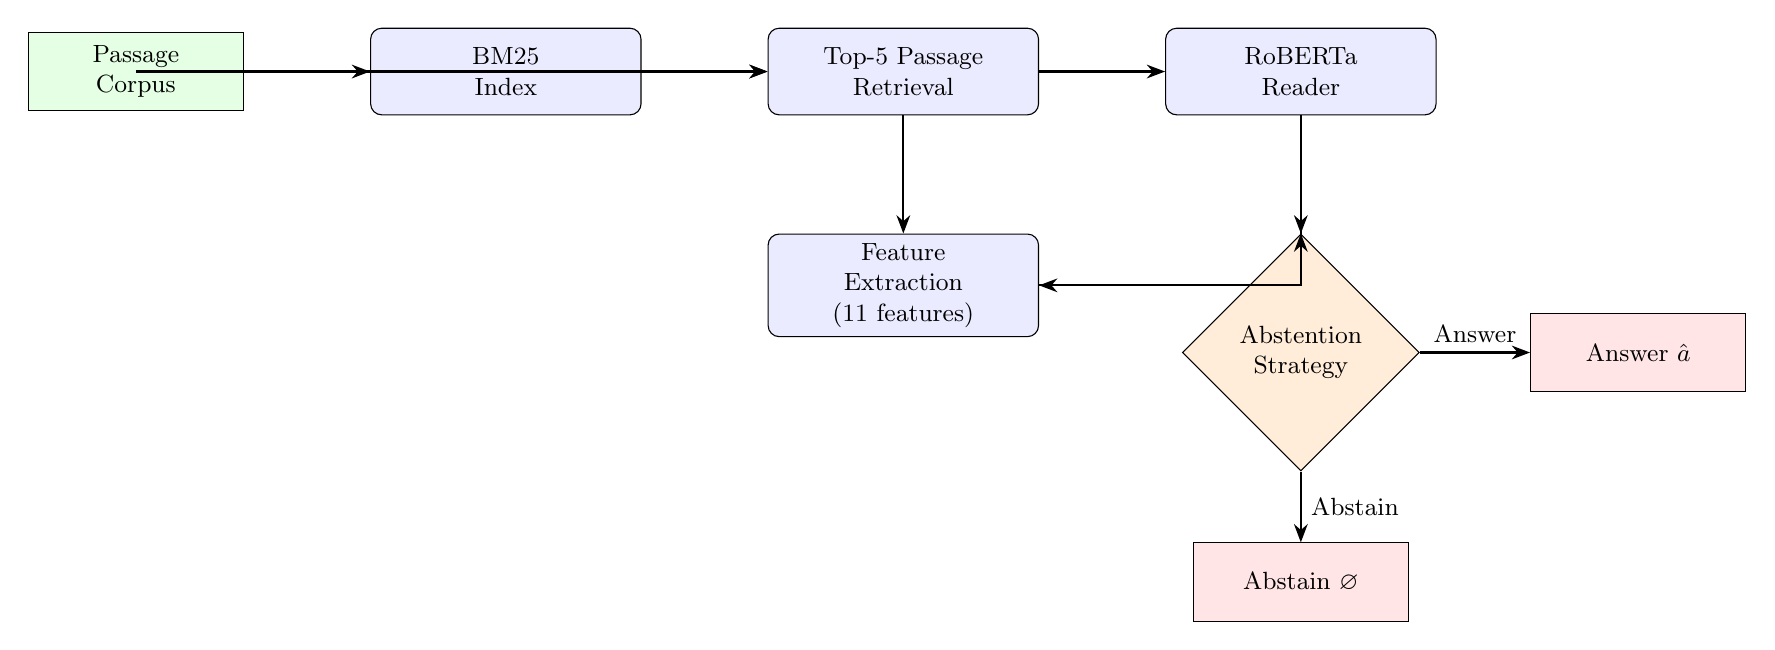
\begin{tikzpicture}[
      node distance = 1.1cm and 1.6cm,
      >=Stealth,
      block/.style = {rectangle, draw, rounded corners=4pt,
                      fill=blue!8, text width=3.2cm,
                      minimum height=1.1cm, align=center,
                      font=\small},
      decision/.style = {diamond, draw, fill=orange!15,
                         text width=2.2cm, align=center,
                         inner sep=1pt, font=\small},
      io/.style     = {rectangle, draw, fill=green!10,
                       text width=2.5cm, minimum height=1cm,
                       align=center, font=\small},
      result/.style = {rectangle, draw, fill=red!10,
                       text width=2.5cm, minimum height=1cm,
                       align=center, font=\small},
      line/.style   = {draw, -Stealth, thick},
    ]

    %% Nodes
    \node[io]       (input)    {Question $q$};
    \node[block,    right=of input]  (bm25idx)  {BM25\\Index};
    \node[block,    right=of bm25idx](retrieval){Top-5 Passage\\Retrieval};
    \node[block,    right=of retrieval](reader){RoBERTa\\Reader};

    %% Feature extraction below retrieval
    \node[block,    below=1.5cm of retrieval](features){Feature\\Extraction\\(11 features)};

    %% Abstention decision
    \node[decision, below=1.5cm of reader](abstain){Abstention\\Strategy};

    %% Outputs
    \node[result,   right=1.4cm of abstain](answer){Answer $\hat{a}$};
    \node[result,   below=0.9cm of abstain](abstain_out){Abstain $\varnothing$};

    %% Corpus
    \node[io, left=of bm25idx](corpus){Passage\\Corpus};

    %% Arrows
    \draw[line] (corpus)    -- (bm25idx);
    \draw[line] (bm25idx)   -- (retrieval);
    \draw[line] (input)     |- (retrieval);
    \draw[line] (retrieval) -- (reader);
    \draw[line] (retrieval) -- (features);
    \draw[line] (reader)    |- (features);
    \draw[line] (reader)    -- (abstain);
    \draw[line] (features)  -| (abstain);
    \draw[line] (abstain)   -- node[above]{\small Answer} (answer);
    \draw[line] (abstain)   -- node[right]{\small Abstain} (abstain_out);

  \end{tikzpicture}
  \caption{End-to-end RAG-with-abstention pipeline. The question is used to
           retrieve passages via BM25, the top-1 passage is passed to the
           RoBERTa reader, and the combined 11-dimensional feature vector is
           evaluated by the abstention strategy to decide whether to answer or
           abstain.}
  \label{fig:architecture}
\end{figure}

\section{Component Interactions and Data Flow}
\label{sec:arch_dataflow}

The pipeline is implemented in Python using the \texttt{rank\_bm25} library for
retrieval and the Hugging Face \texttt{transformers} library for the QA reader.
Feature vectors are stored as \texttt{pandas} DataFrames and serialised to CSV
files after each pipeline stage, enabling reproducibility and offline analysis.

\paragraph{BM25 $\rightarrow$ Features.}
After retrieval, the \texttt{top\_bm25\_score}, \texttt{second\_bm25\_score},
\texttt{bm25\_score\_gap}, \texttt{mean\_topk\_bm25}, and
\texttt{source\_passage\_retrieved} features are computed directly from the
ranked list of (score, passage) pairs. These five values, together with the
question metadata features (\texttt{question\_length}, \texttt{question\_token\_count}),
are available before the reader is invoked.

\paragraph{Reader $\rightarrow$ Features.}
The reader's outputs (\texttt{qa\_score}, \texttt{qa\_no\_answer\_probability},
\texttt{predicted\_answer\_length}, \texttt{answer\_nonempty}) are appended to
the feature vector after the reader processes the top-1 passage.

\paragraph{Classifier Training.}
During training, the full 11-feature vectors are labelled with the ground-truth
answerability flag and used to fit the logistic regression classifier. The
trained model and its fitted \texttt{StandardScaler}+\texttt{SimpleImputer}
pre-processors are saved to disk and loaded at test time.

\paragraph{Threshold Selection.}
Both the BM25 threshold $\tau$ and the classifier threshold $\delta$ are
selected by sweeping candidate values on the validation set, measuring F1, and
picking the maximiser. The best classifier threshold found is $\delta^* = 0.28$.
Only then are the thresholds applied to the held-out test set.

\section{Design Principles}
\label{sec:arch_principles}

Several design principles guided the architecture:

\begin{description}
  \item[Modularity.] Each stage produces a well-defined output artifact (CSV
        file or pickled model), allowing stages to be run independently and
        results to be reproduced without re-running the entire pipeline.

  \item[Leakage prevention.] BM25 indices are built per-split; the classifier
        is trained only on training features; thresholds are tuned only on
        validation features. The test set remains entirely held out.

  \item[Interpretability.] The choice of logistic regression over a black-box
        model is deliberate: the learned coefficients can be inspected to
        understand which features most influence the abstention decision.

  \item[Scalability considerations.] While BM25 is efficient at corpus scale,
        the architecture is designed so that the retrieval backbone can be
        swapped for a dense retriever (e.g., DPR) without changing the
        downstream feature extraction or classifier code.
\end{description}

%% ============================================================
%% Chapter 5 — Experimental Setup
%% ============================================================
\chapter{Experimental Setup}
\label{chap:experiments}

\section{Dataset Statistics}
\label{sec:exp_data_stats}

Table~\ref{tab:dataset_stats} summarises the final article-level split.
Figure~\ref{fig:dataset_distribution} provides a visual breakdown. All three
splits are perfectly balanced between answerable and unanswerable questions,
ensuring that a trivial strategy of always answering achieves exactly 50\%
precision when measured on answerability—not 100\%—and that evaluation metrics
are interpretable without correction for class imbalance.

\begin{table}[htbp]
  \centering
  \caption{Dataset split statistics for SQuAD~2.0 (article-level split, seed 42).}
  \label{tab:dataset_stats}
  \begin{tabular}{lrrrr}
    \toprule
    \textbf{Split} & \textbf{Total} & \textbf{Answerable} & \textbf{Unanswerable} & \textbf{Articles} \\
    \midrule
    Train      & 300 & 150 & 150 & 176 \\
    Validation & 100 &  50 &  50 &  61 \\
    Test       & 100 &  50 &  50 &  55 \\
    \midrule
    \textbf{Total} & \textbf{500} & \textbf{250} & \textbf{250} & \textbf{292} \\
    \bottomrule
  \end{tabular}
\end{table}

\begin{figure}[htbp]
  \centering
  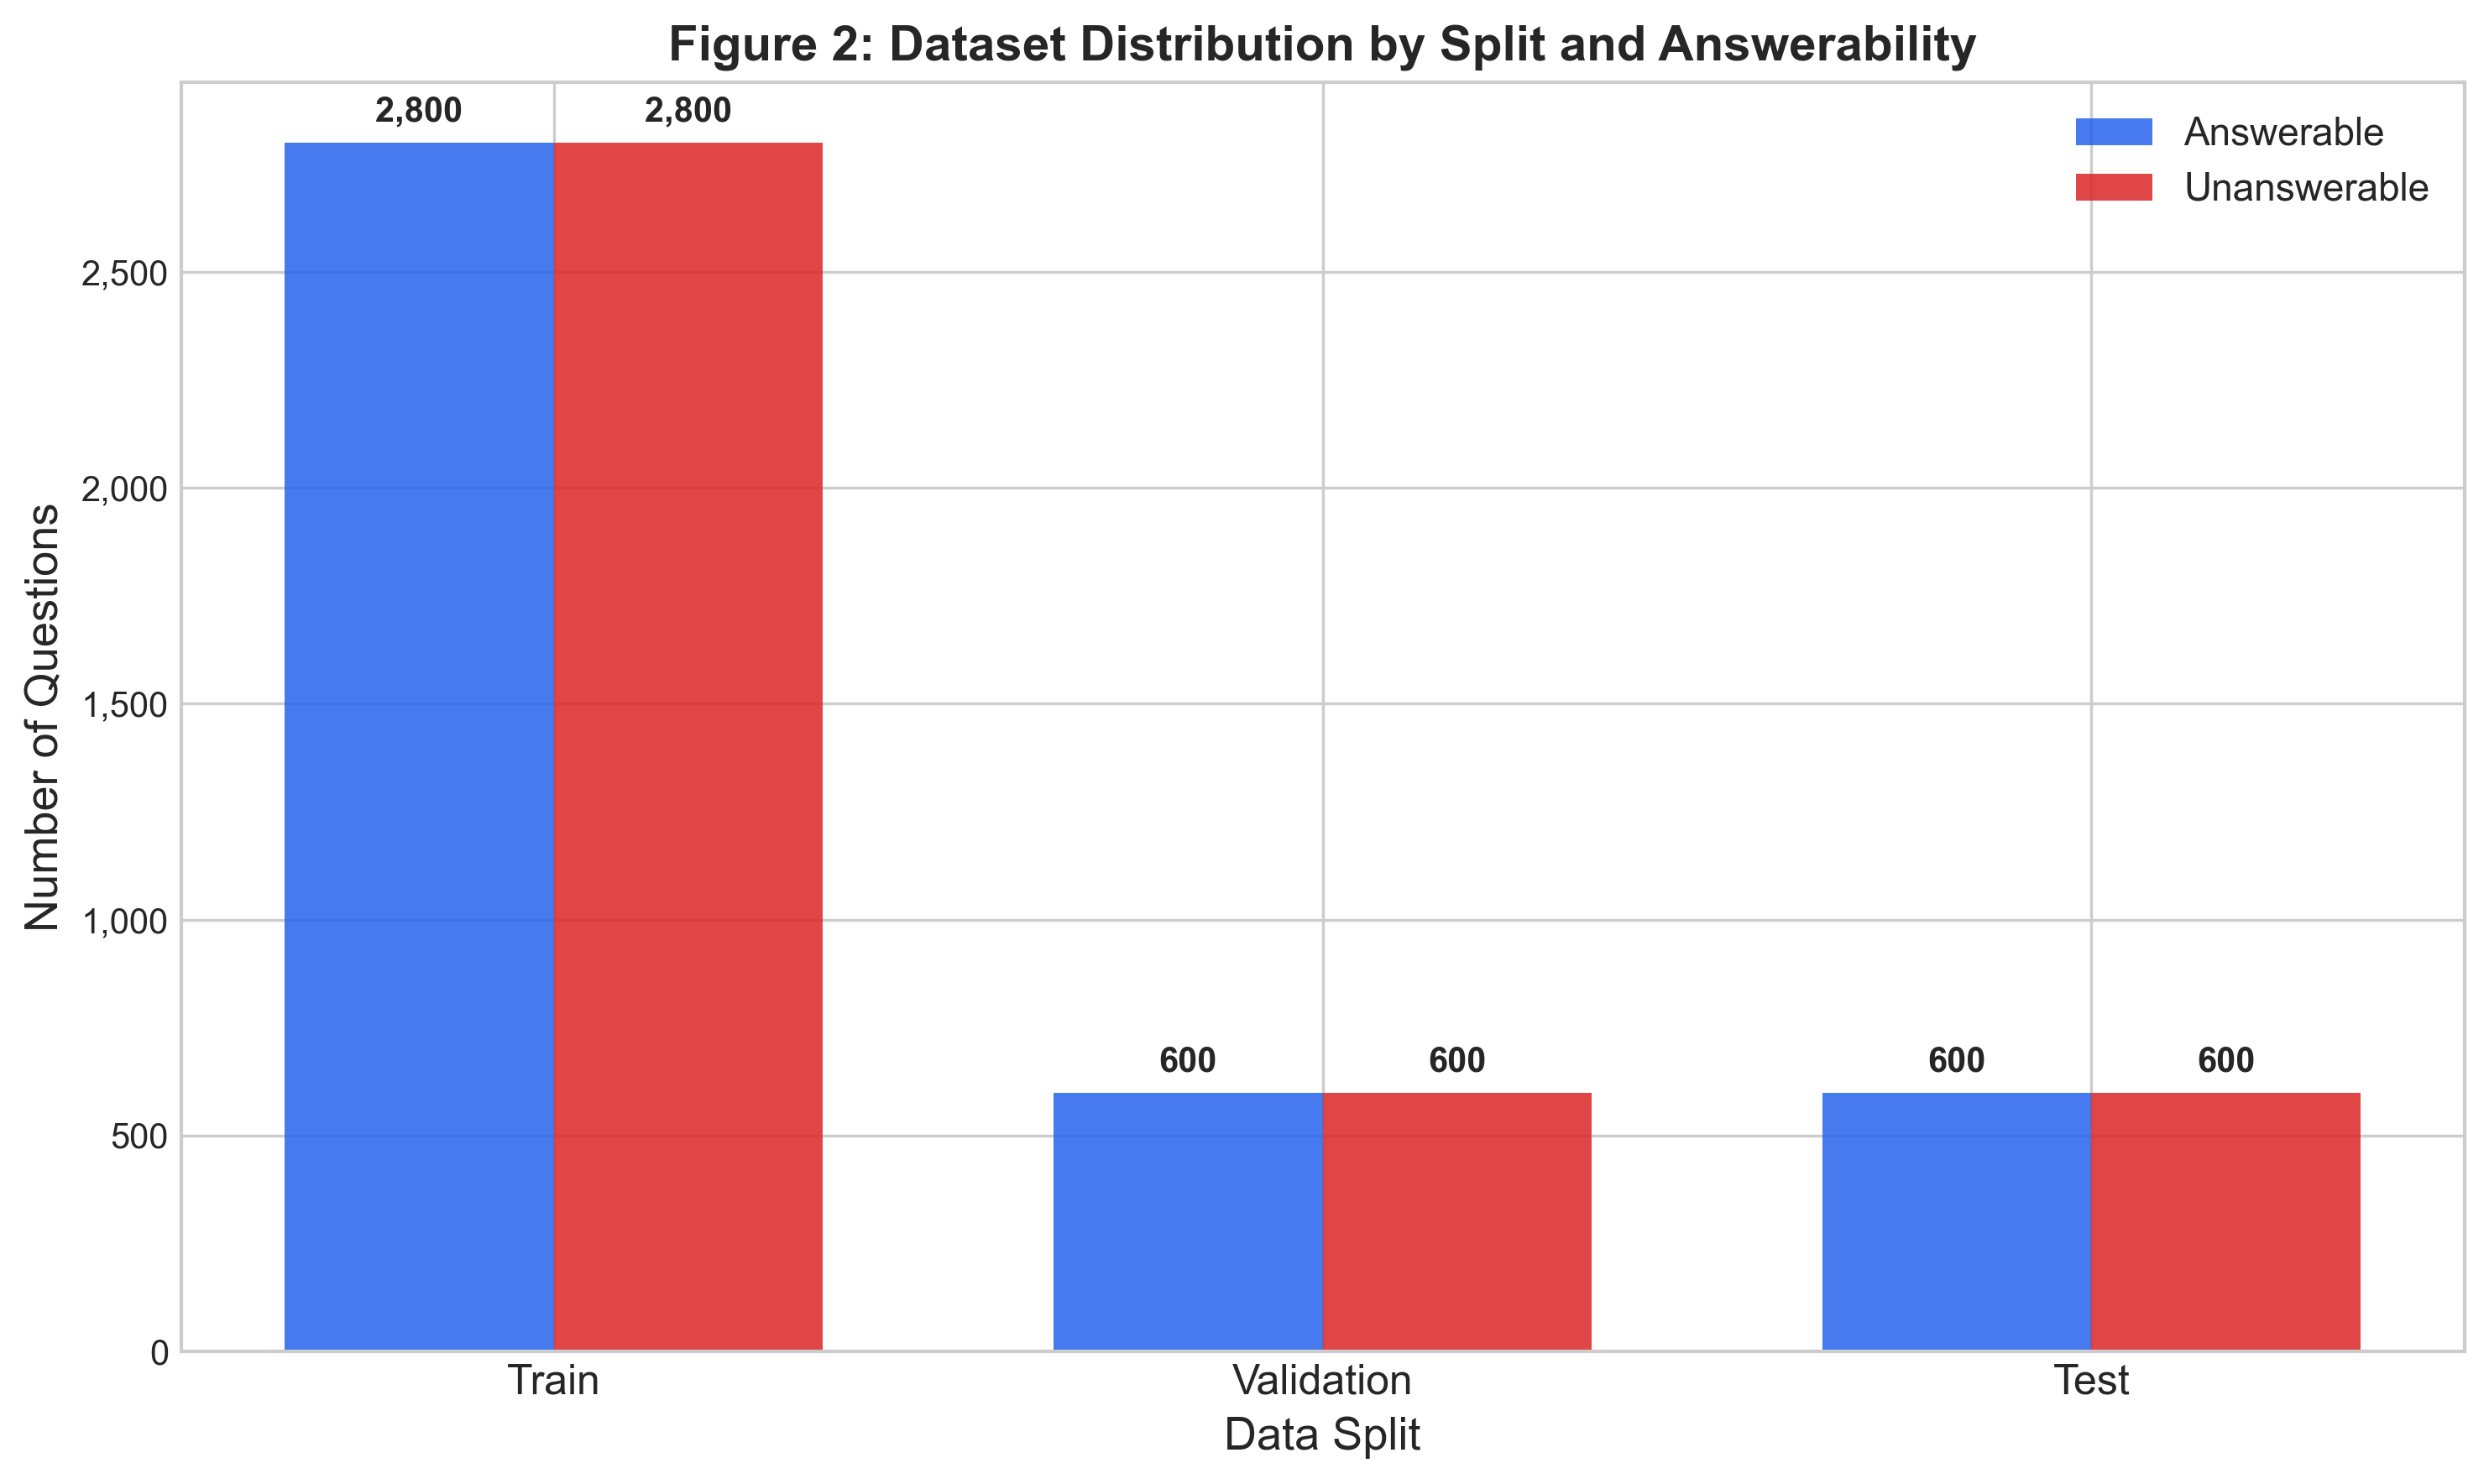
\includegraphics[width=0.80\textwidth]{fig2_dataset_distribution}
  \caption{Answerable vs.\ unanswerable question counts per data split.}
  \label{fig:dataset_distribution}
\end{figure}

\section{BM25 Configuration}
\label{sec:exp_bm25_config}

We use the \texttt{rank\_bm25} Python package (Okapi BM25 variant) with
default hyper-parameters: $k_1 = 1.5$, $b = 0.75$. Text is lower-cased and
split on whitespace before indexing. The top-$k = 5$ passages are retrieved
per query. Table~\ref{tab:bm25_stats} shows descriptive statistics for the
top-BM25-score feature across splits.

\begin{table}[htbp]
  \centering
  \caption{Descriptive statistics of \texttt{top\_bm25\_score} by data split.}
  \label{tab:bm25_stats}
  \begin{tabular}{lrrrr}
    \toprule
    \textbf{Split} & \textbf{Mean} & \textbf{Std} & \textbf{Min} & \textbf{Max} \\
    \midrule
    Train      & 30.89 & 13.13 &  4.49 & 107.21 \\
    Validation & 26.60 & 11.45 &  5.95 &  82.57 \\
    Test       & 26.69 & 12.02 &  4.98 & 112.81 \\
    \bottomrule
  \end{tabular}
\end{table}

Figures~\ref{fig:bm25_distribution} and \ref{fig:bm25_per_split} visualise the
BM25 score distributions by answerability label and by split, respectively.

\begin{figure}[htbp]
  \centering
  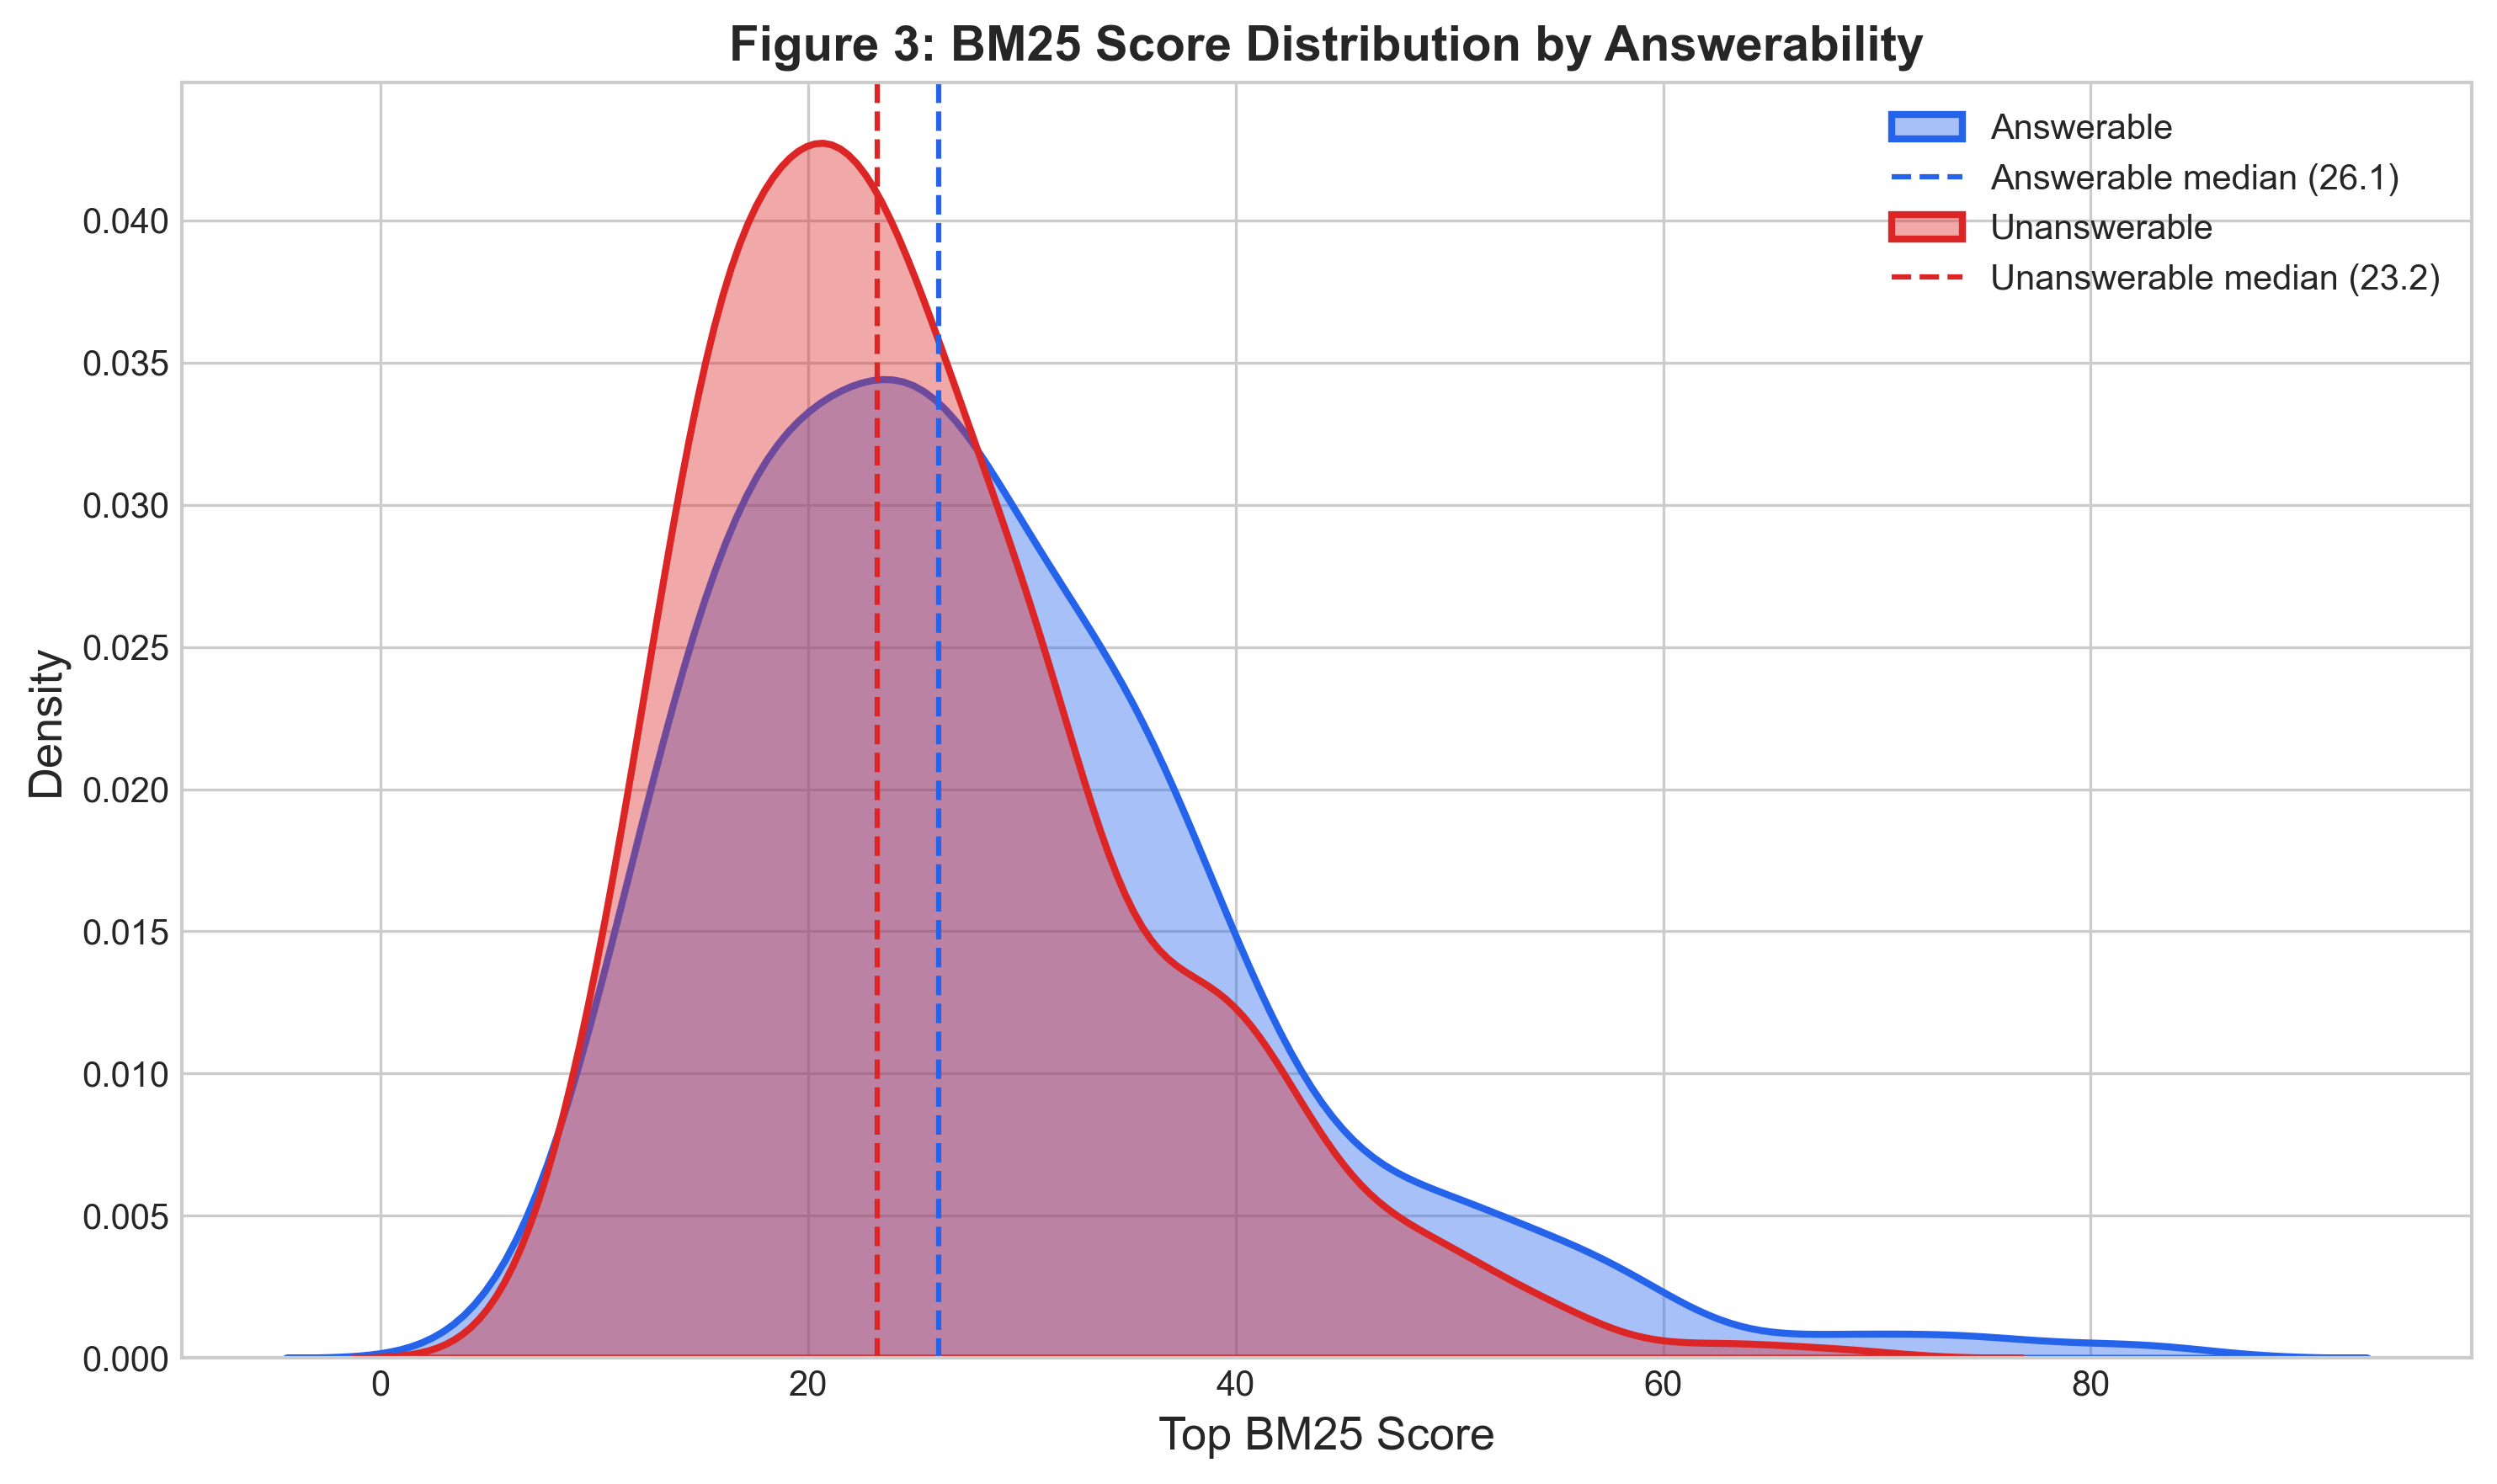
\includegraphics[width=0.80\textwidth]{fig3_bm25_score_distribution}
  \caption{Distribution of \texttt{top\_bm25\_score} for answerable vs.\
           unanswerable questions on the validation split.}
  \label{fig:bm25_distribution}
\end{figure}

\begin{figure}[htbp]
  \centering
  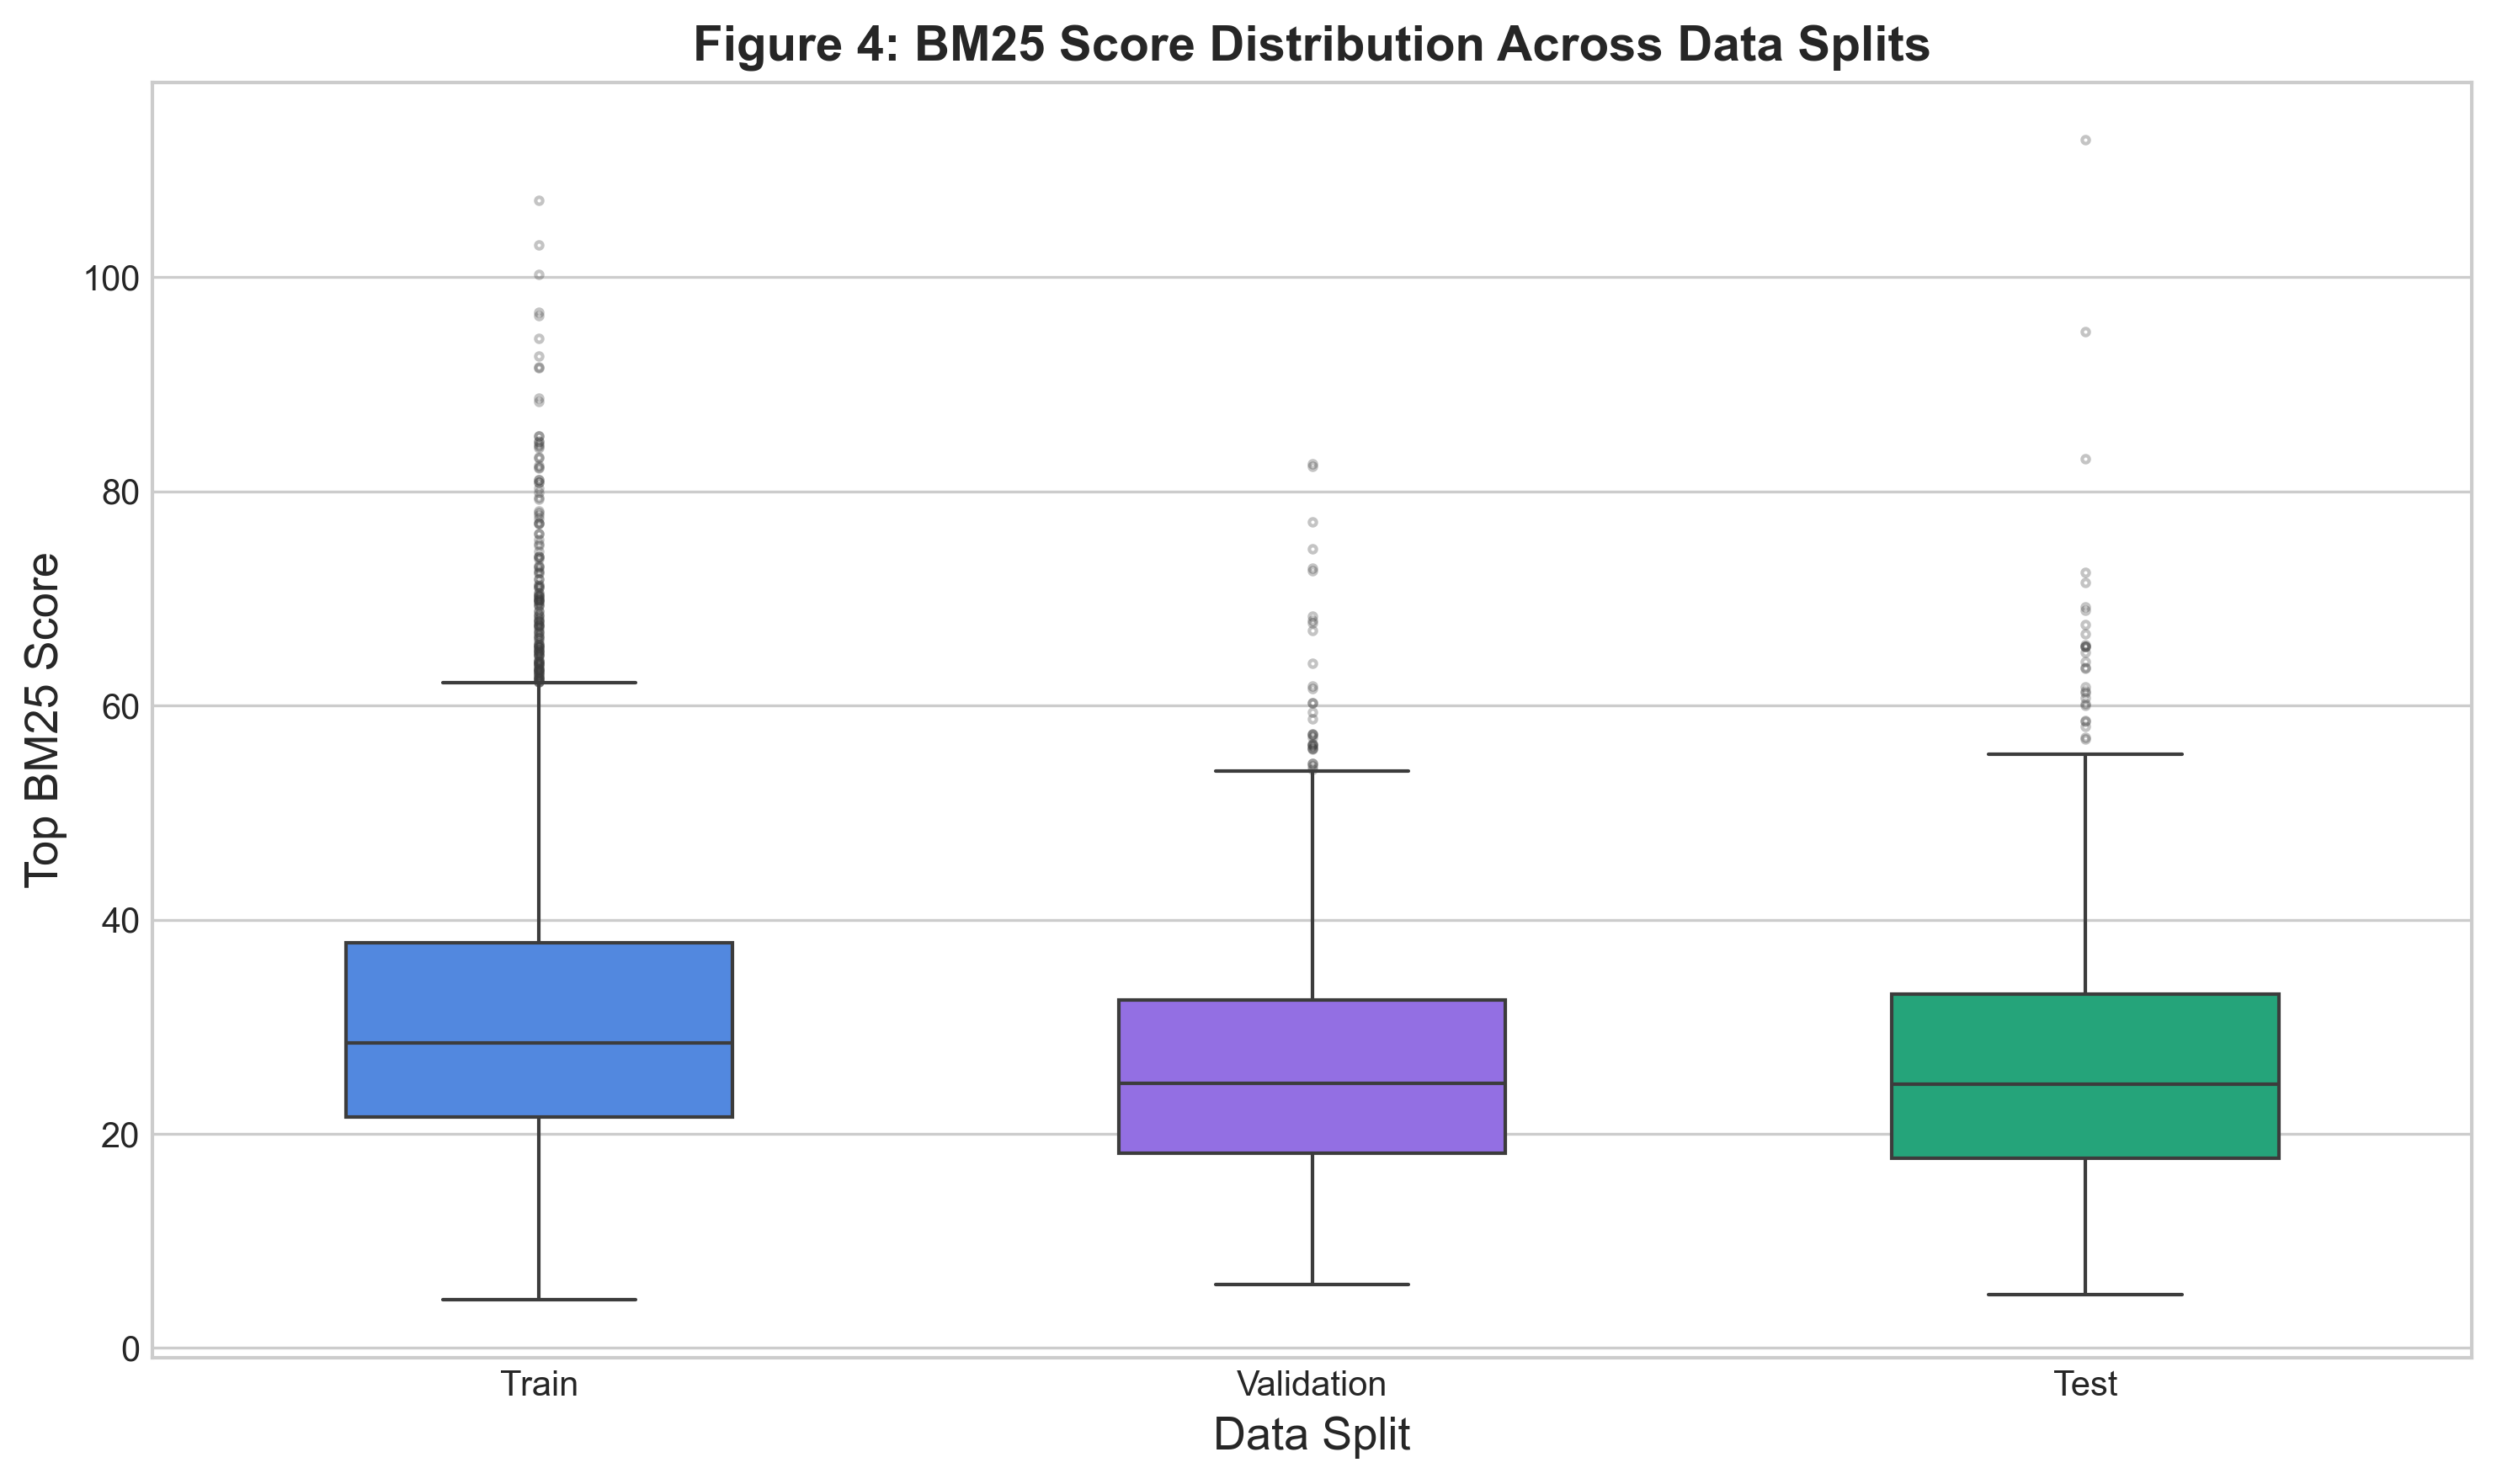
\includegraphics[width=0.80\textwidth]{fig4_bm25_scores_per_split}
  \caption{Box plots of \texttt{top\_bm25\_score} across data splits.}
  \label{fig:bm25_per_split}
\end{figure}

\section{QA Reader Configuration}
\label{sec:exp_reader_config}

\begin{itemize}
  \item \textbf{Model checkpoint:} \texttt{deepset/roberta-base-squad2} (Hugging
        Face Hub).
  \item \textbf{Task:} \texttt{question-answering} pipeline.
  \item \textbf{handle\_impossible\_answer:} \texttt{True}.
  \item \textbf{Passages per question:} 1 (top-1 BM25 result only).
  \item \textbf{Device:} CPU (or GPU if available; inference results are
        deterministic).
  \item \textbf{Max sequence length:} 512 tokens (model default).
\end{itemize}

On the test set, the \texttt{qa\_score} has mean $0.290$ ($\sigma = 0.365$),
ranging from near-zero to $0.996$, reflecting the range from clearly
unanswerable questions (low score) to highly confident extractable answers
(high score).

\section{Classifier Configuration}
\label{sec:exp_classifier_config}

\begin{itemize}
  \item \textbf{Model:} \texttt{LogisticRegression} (\texttt{sklearn}).
  \item \textbf{Solver:} LBFGS, maximum 2,000 iterations, balanced class weighting.
  \item \textbf{Regularisation:} L2, $C = 1.0$.
  \item \textbf{Pre-processing:} \texttt{SimpleImputer} (median strategy) $\rightarrow$
        \texttt{StandardScaler}.
  \item \textbf{Features:} 10 inference features (see Table~\ref{tab:features}).
  \item \textbf{Training data:} 300 training questions.
  \item \textbf{Threshold search:} $\delta \in [0.01, 0.99]$ step 0.01 on
        validation set (100 questions); best $\delta^* = 0.42$ ($\tau_{\text{BM25}} = 13.15$).
\end{itemize}

\section{Evaluation Protocol}
\label{sec:exp_eval_protocol}

For each question, the ground-truth label is \emph{answerable} (1) if
\texttt{is\_impossible}~$= 0$, else \emph{unanswerable} (0). An answer is
considered \emph{correct} if the system returns a non-empty string when the
question is answerable, or returns empty / abstains when the question is
unanswerable.

We compute the six metrics defined in Section~\ref{sec:meth_metrics}
(Precision, Recall, F1, Coverage, False-Answer Rate, False-Abstention Rate) on
the test set for each of the three strategies. The BM25 threshold and
classifier threshold are fixed to validation-tuned values before the test set
is evaluated. All computations are reproduced from the \texttt{results/}
directory using the saved prediction and decision CSV files.

%% ============================================================
%% Chapter 6 — Results
%% ============================================================
\chapter{Results}
\label{chap:results}

\section{Strategy Comparison on the Test Set}
\label{sec:results_comparison}

Table~\ref{tab:strategy_comparison} summarises the performance of all three
strategies on the held-out test set of 1,200 questions. All hyper-parameters
were fixed prior to evaluation using the validation set only.

\begin{table}[htbp]
  \centering
  \caption{Abstention strategy comparison on the test set
           (1,200 questions: 600 answerable, 600 unanswerable).}
  \label{tab:strategy_comparison}
  \begin{tabular}{lcccccc}
    \toprule
    \textbf{Strategy} &
    \textbf{Precision} & \textbf{Recall} & \textbf{F1} &
    \textbf{Coverage} & \textbf{FAR} & \textbf{FAbR} \\
    \midrule
    Always Answer               & 0.4820 & 1.0000 & 0.6505 & 1.000 & 1.0000 & 0.0000 \\
    BM25 Threshold              & 0.4810 & 0.9959 & 0.6486 & 0.998 & 1.0000 & 0.0042 \\
    Answerability Classifier    & \textbf{0.8231} & 0.8880 & \textbf{0.8543} & 0.520 & \textbf{0.1776} & 0.1120 \\
    \bottomrule
    \multicolumn{7}{l}{\small FAR = False-Answer Rate; FAbR = False-Abstention Rate.} \\
    \multicolumn{7}{l}{\small Bold = best value in column.} \\
  \end{tabular}
\end{table}

\begin{figure}[htbp]
  \centering
  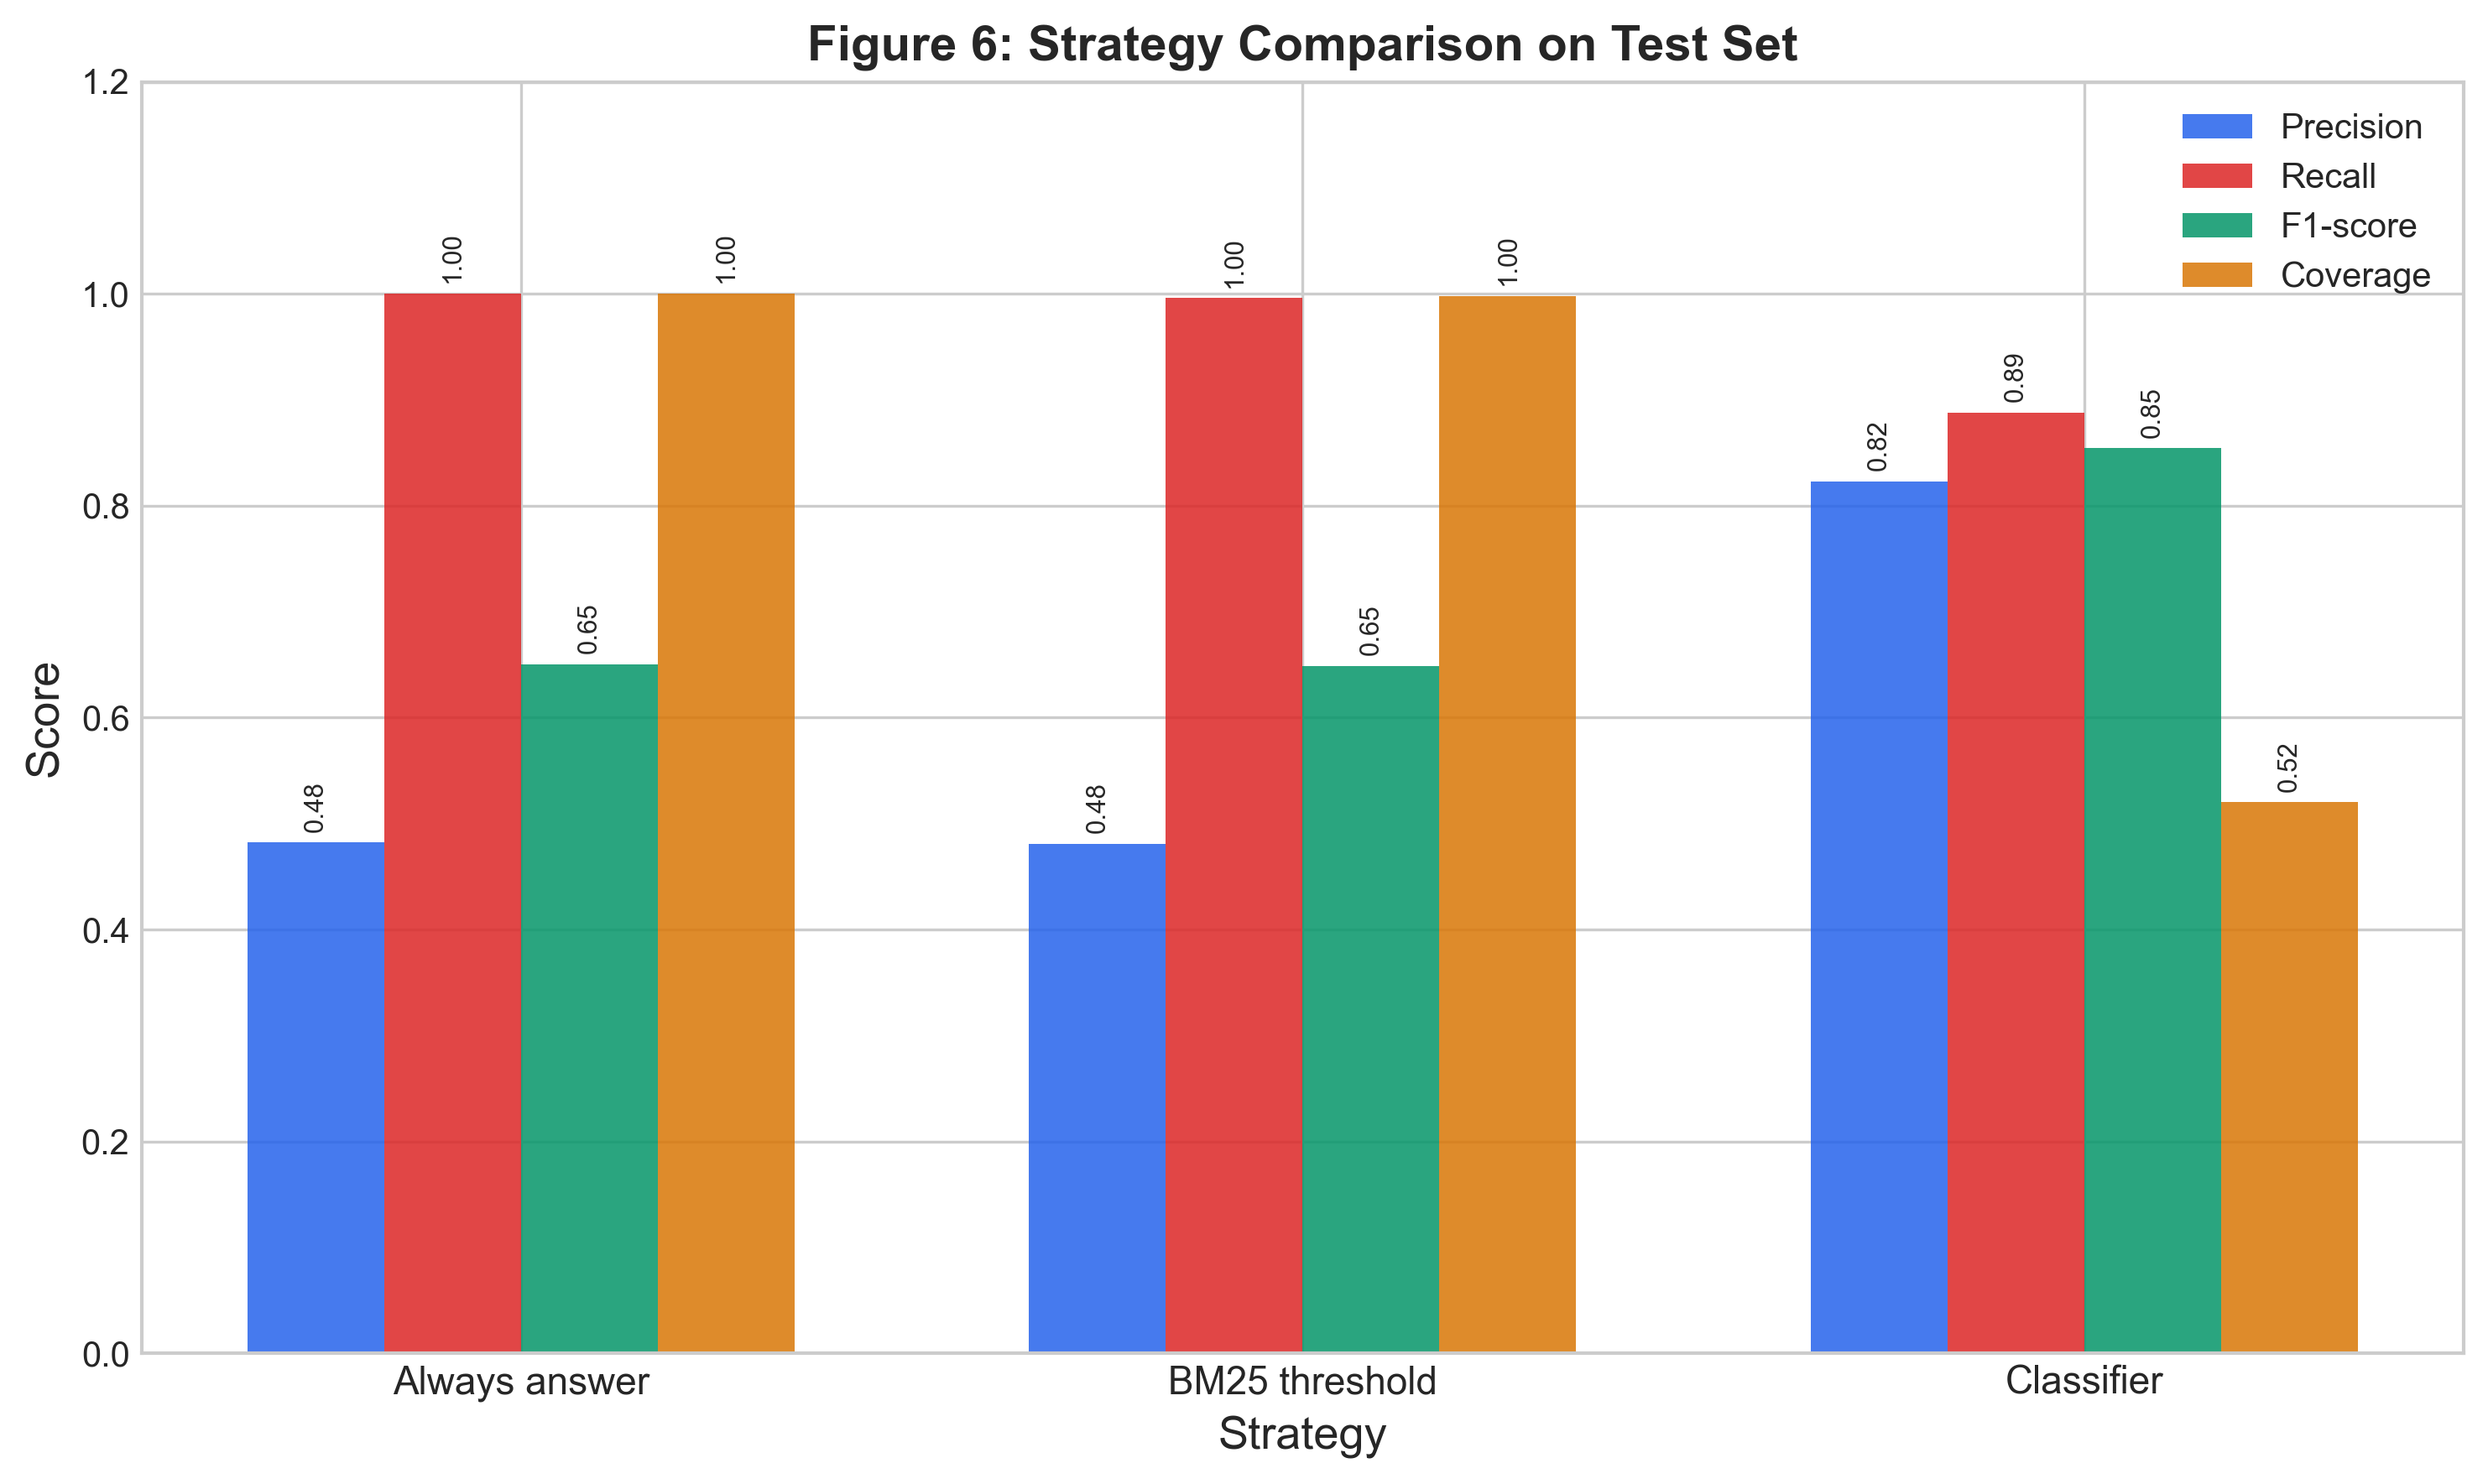
\includegraphics[width=0.80\textwidth]{fig6_strategy_comparison}
  \caption{Grouped bar chart comparing Precision, Recall, F1 and Coverage
           across the three abstention strategies on the test set.}
  \label{fig:strategy_comparison}
\end{figure}

\section{Interpretation}
\label{sec:results_interpretation}

\paragraph{Always Answer (Baseline).}
By design, this strategy achieves perfect recall ($= 1.00$) and perfect
coverage ($= 1.00$), since it never abstains. However, its precision is only
0.4820—barely above the random 50\% baseline on a balanced dataset—and its
False-Answer Rate is 1.00, meaning it provides a spurious answer to every
unanswerable question. The resulting F1 of 0.6505 reflects the fundamental
tension: high coverage is purchased at the cost of extreme imprecision on
unanswerable questions.

\paragraph{BM25 Threshold.}
The BM25 Threshold strategy (optimal validation-tuned $\tau$) achieves nearly
identical metrics to the baseline: precision 0.4810, F1 0.6486, and
False-Answer Rate 1.00. Coverage falls marginally to 0.998, meaning only 2.4
questions out of 1,200 are suppressed (2 questions, in absolute terms). This
result is striking: a single BM25 score threshold is essentially \emph{unable}
to discriminate answerable from unanswerable questions at the score levels
produced by the retriever over this dataset. The near-identical performance to
the baseline suggests that \emph{BM25 score alone is a poor abstention signal}
when used as a simple threshold.

\paragraph{Answerability Classifier.}
The logistic regression classifier achieves substantially superior results:
precision 0.8231, recall 0.8880, and F1 0.8543. These are improvements of
+34.1 pp in precision and +19.4 pp in F1 over the best single-threshold
strategy. The False-Answer Rate drops dramatically from 1.00 to 0.1776,
meaning the system now correctly abstains on approximately 82\% of unanswerable
questions.

The cost is a reduced coverage of 0.520: the classifier chooses to answer
only 52\% of questions (624 out of 1,200), and of those it abstains on, 11.2\%
are actually answerable (False-Abstention Rate = 0.1120). Whether this
precision–coverage trade-off is acceptable depends on the deployment context:
in high-stakes settings, a 82\% reduction in false answers at the cost of
answering only half of questions is likely worthwhile.

\section{Threshold Selection}
\label{sec:results_threshold}

Figure~\ref{fig:threshold_selection} shows precision, recall, and F1 as
functions of the classifier probability threshold $\delta$ on the validation
set. The optimal threshold $\delta^* = 0.28$ lies well below 0.5, reflecting
the fact that the classifier's default operating point (argmax) is biased
toward answering, and a lower threshold is needed to push recall at the cost of
precision.

\begin{figure}[htbp]
  \centering
  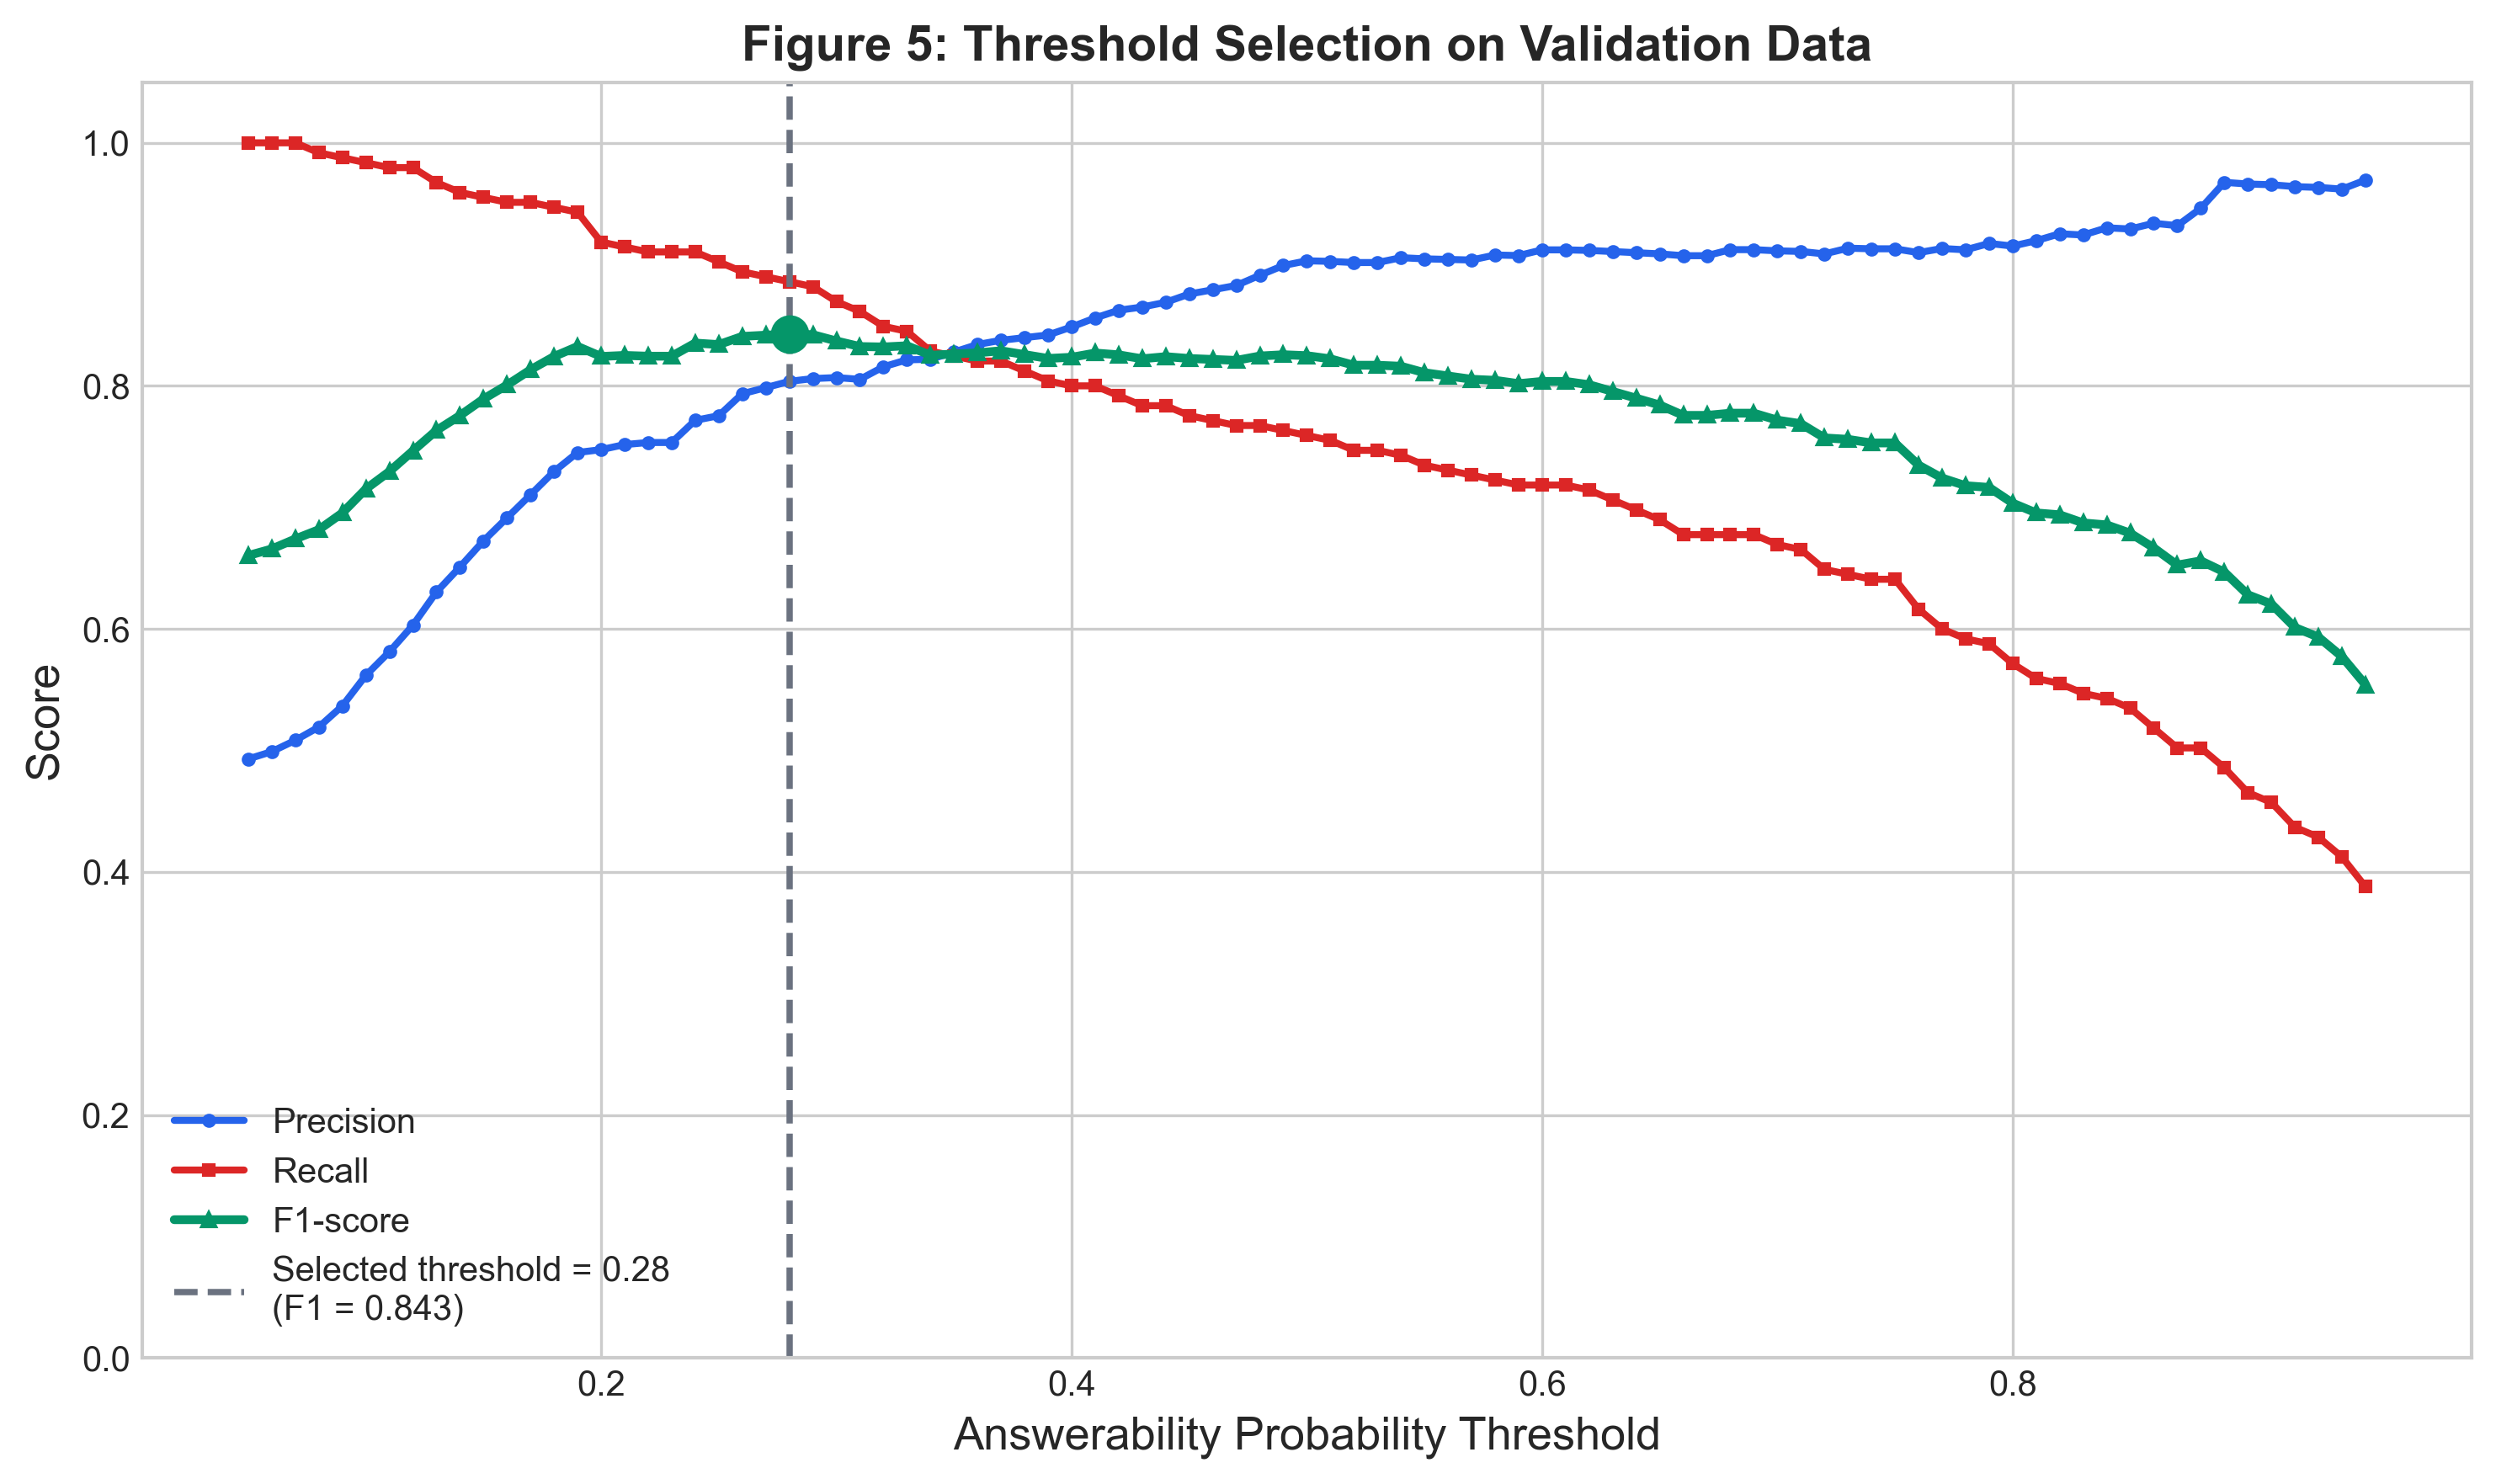
\includegraphics[width=0.80\textwidth]{fig5_threshold_selection}
  \caption{Precision, Recall, and F1 as functions of the classifier probability
           threshold on the validation set. The vertical dashed line marks the
           selected threshold $\delta^* = 0.28$.}
  \label{fig:threshold_selection}
\end{figure}

\section{Classifier Performance}
\label{sec:results_classifier}

Table~\ref{tab:classifier_performance} reports the classifier's binary
answerability prediction performance on the test set, treating the problem as
a binary classification task (answerable vs.\ unanswerable). The applied
threshold is $\delta^* = 0.28$.

\begin{table}[htbp]
  \centering
  \caption{Answerability classifier performance on the test set
           at threshold $\delta^* = 0.28$.}
  \label{tab:classifier_performance}
  \begin{tabular}{lcccc}
    \toprule
    \textbf{Set} & \textbf{Precision} & \textbf{Recall} & \textbf{F1} & \textbf{Accuracy} \\
    \midrule
    Test  & 0.8231 & 0.8880 & 0.8543 & 0.8540 \\
    \bottomrule
  \end{tabular}
\end{table}

\subsection{Confusion Matrix}

Figure~\ref{fig:confusion_matrix} and Table~\ref{tab:confusion_matrix} show the
confusion matrix on the test set.

\begin{table}[htbp]
  \centering
  \caption{Classifier confusion matrix on the test set.}
  \label{tab:confusion_matrix}
  \begin{tabular}{lcc}
    \toprule
    & \textbf{Predicted: Abstain} & \textbf{Predicted: Answer} \\
    \midrule
    \textbf{Actual: Unanswerable} & 213 (TN) & 46 (FP) \\
    \textbf{Actual: Answerable}   &  27 (FN) & 214 (TP) \\
    \bottomrule
  \end{tabular}
\end{table}

\begin{figure}[htbp]
  \centering
  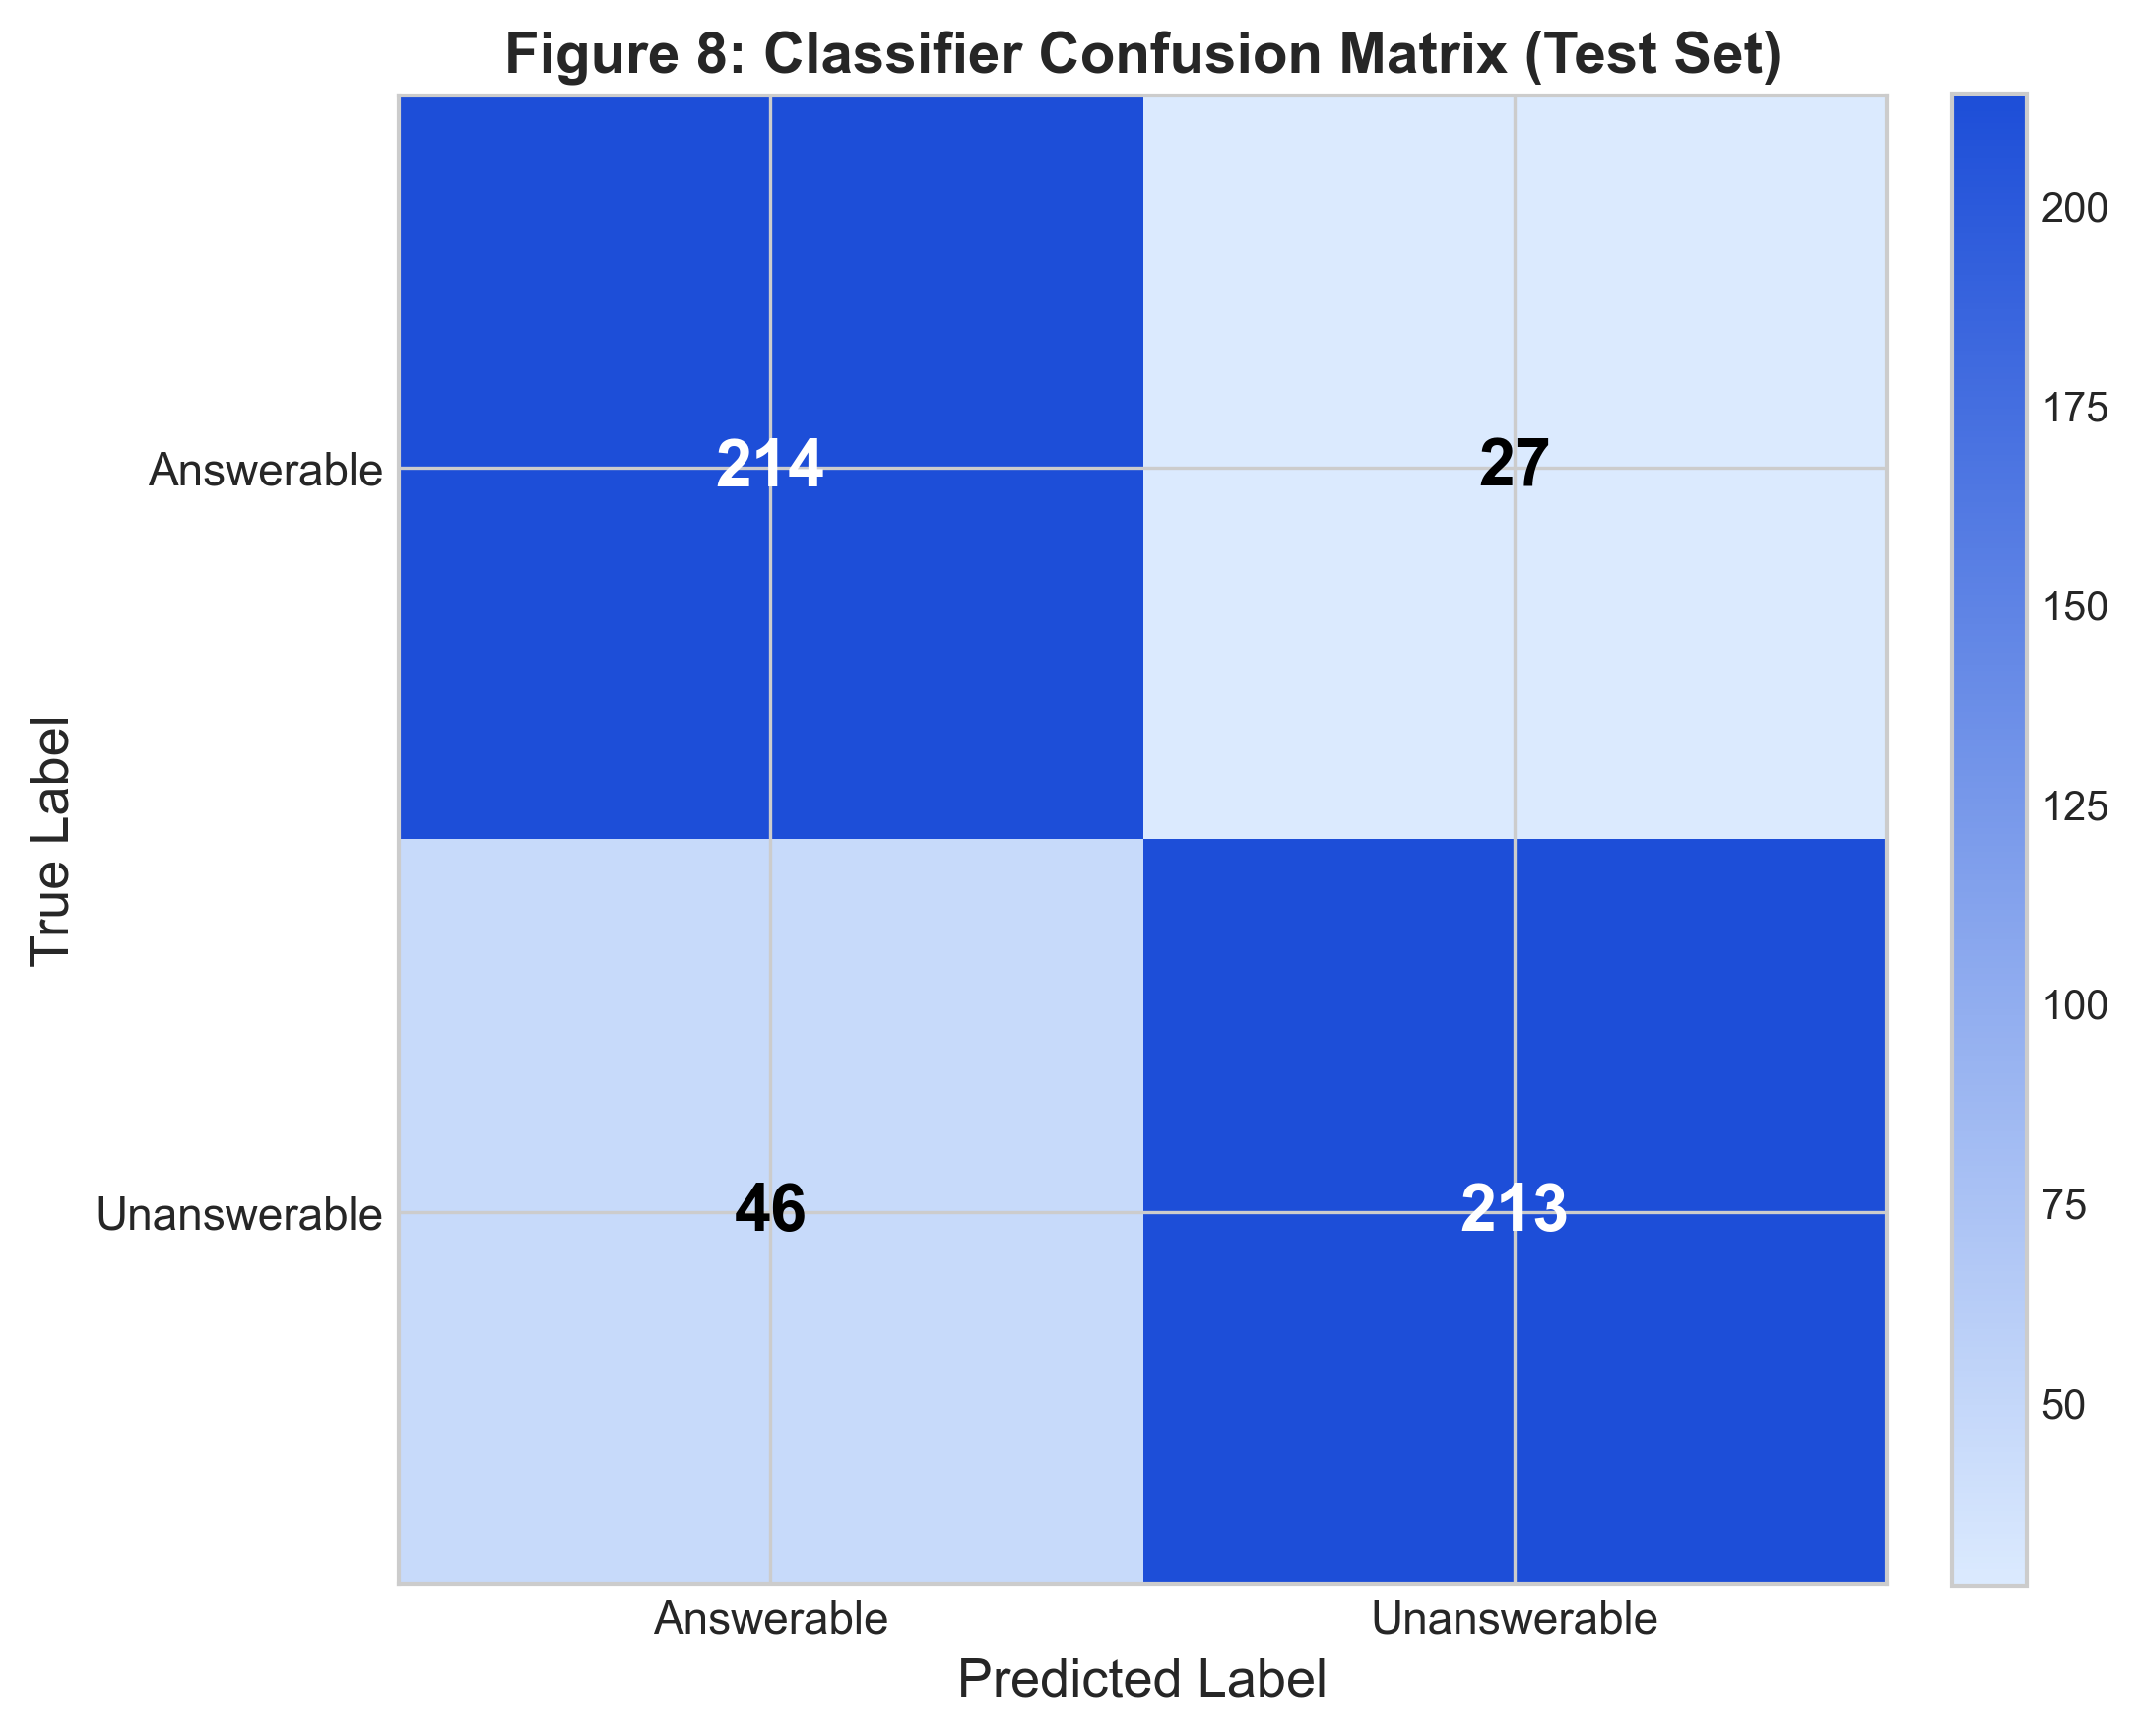
\includegraphics[width=0.60\textwidth]{fig8_confusion_matrix}
  \caption{Confusion matrix of the answerability classifier on the test set.
           TN = True Negative (correctly abstained), FP = False Positive (answered
           an unanswerable question), FN = False Negative (abstained on an
           answerable question), TP = True Positive (correctly answered).}
  \label{fig:confusion_matrix}
\end{figure}

The confusion matrix reveals an asymmetry: the classifier makes
$\text{FP} = 46$ errors (answering unanswerable questions) compared to
$\text{FN} = 27$ errors (abstaining on answerable ones). Given the threshold
$\delta^* = 0.28 < 0.5$, this is expected: the classifier is biased toward
answering, as false abstentions (FN) are penalised more under the F1 objective
used for threshold selection.

\section{Error Analysis Figures}
\label{sec:results_error_fig}

Figure~\ref{fig:error_analysis} shows the breakdown of correct answers,
correct abstentions, false answers, and false abstentions for each strategy,
providing an intuitive comparison of error profiles.

\begin{figure}[htbp]
  \centering
  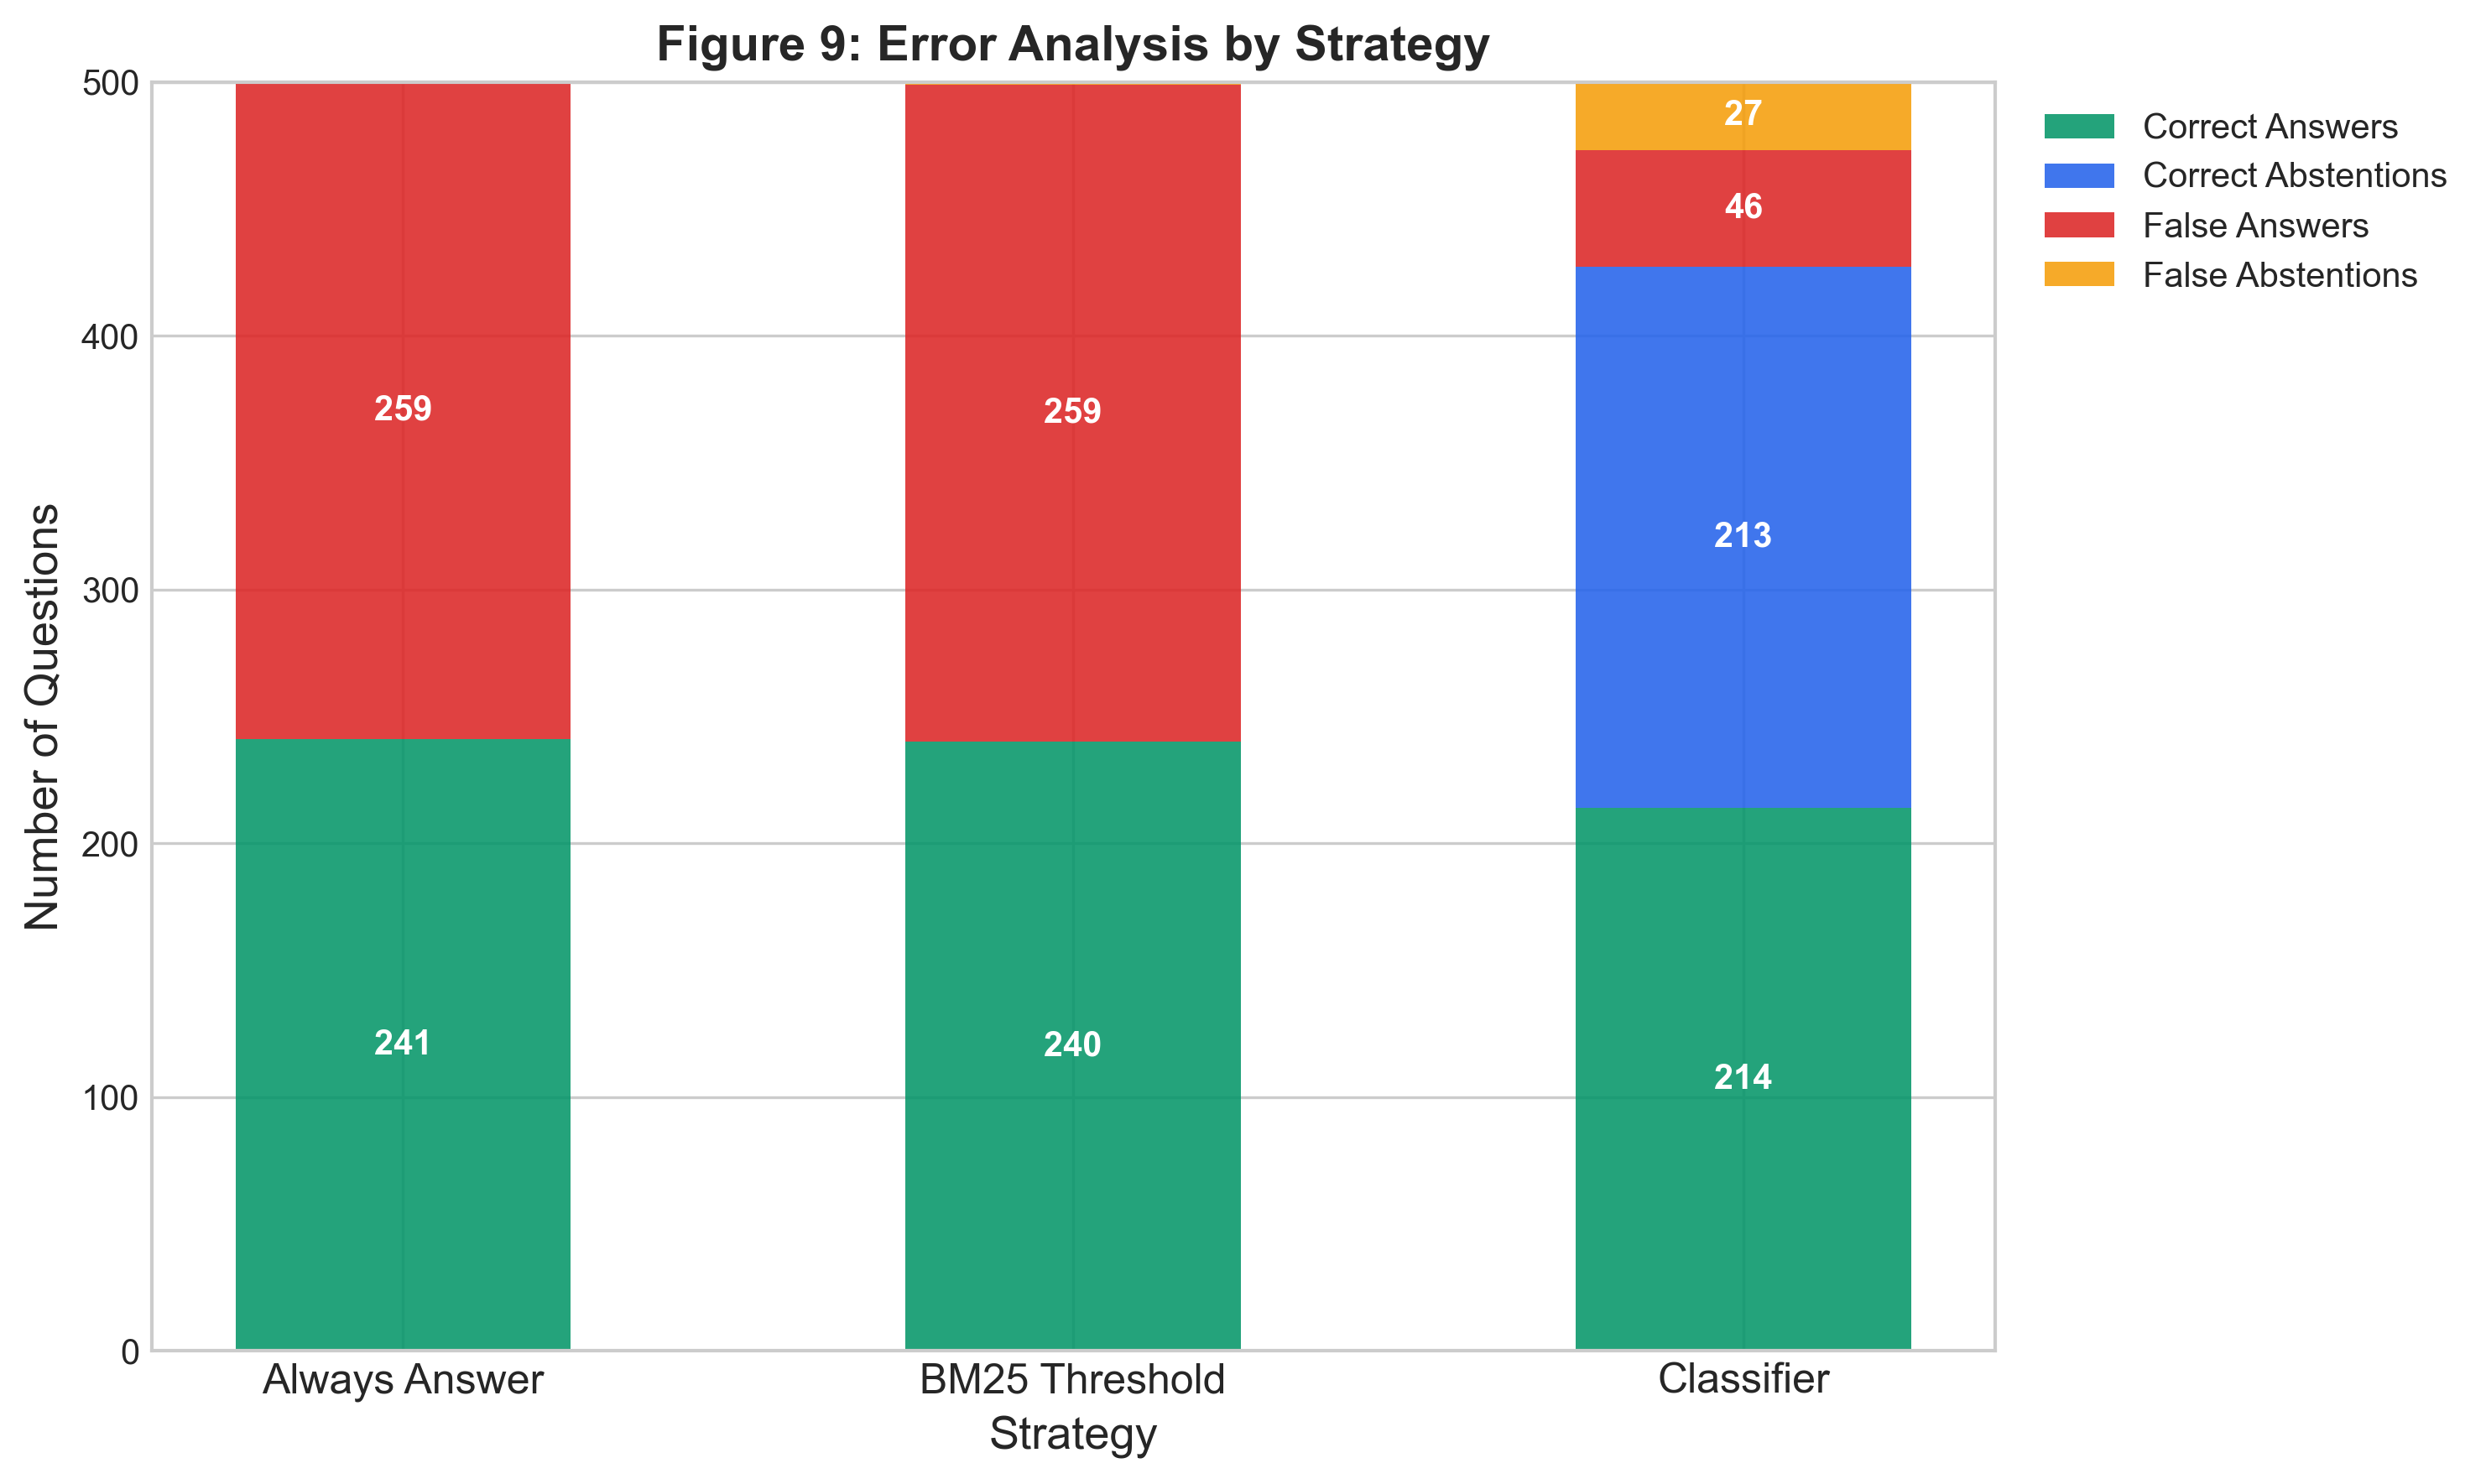
\includegraphics[width=0.80\textwidth]{fig9_error_analysis}
  \caption{Per-strategy breakdown of outcome types on the test set:
           Correct Answer, Correct Abstention, False Answer (answered when should
           have abstained), and False Abstention (abstained when should have
           answered).}
  \label{fig:error_analysis}
\end{figure}

%% ============================================================
%% Chapter 7 — Error Analysis
%% ============================================================
\chapter{Error Analysis}
\label{chap:error_analysis}

\section{Error Taxonomy}
\label{sec:err_taxonomy}

We categorise errors made by the Answerability Classifier into three
orthogonal failure modes. Table~\ref{tab:error_taxonomy} provides a structured
overview; Sections~\ref{sec:err_retrieval}–\ref{sec:err_classification} discuss
each in detail.

\begin{table}[htbp]
  \centering
  \caption{Error taxonomy for the RAG-with-abstention pipeline.}
  \label{tab:error_taxonomy}
  \begin{tabular}{llp{6.5cm}}
    \toprule
    \textbf{Error Type} & \textbf{Locus} & \textbf{Description} \\
    \midrule
    Retrieval Failure      & BM25 retriever  & The ground-truth passage is not in
                                               the top-$k$ results; the reader
                                               has no access to relevant text. \\
    Extraction Failure     & RoBERTa reader  & The ground-truth passage is retrieved,
                                               but the reader extracts an incorrect
                                               or empty span. \\
    Classification Failure & Abstention layer & The classifier makes the wrong
                                               abstention decision regardless of
                                               retrieval and extraction quality. \\
    \bottomrule
  \end{tabular}
\end{table}

\subsection{Retrieval Failure}
\label{sec:err_retrieval}

Retrieval failures arise when BM25 cannot surface the relevant passage among the
top-$k$ results. This happens most often when:

\begin{itemize}
  \item The question contains synonyms or paraphrases not present in the
        passage (lexical mismatch).
  \item The question is about a rare entity that appears in many passages,
        causing relevant passages to be outranked by topically similar but
        factually different ones.
  \item The passage is very short and receives a low BM25 score due to length
        normalisation, even if it is the most relevant.
\end{itemize}

\noindent \textbf{Example.} Consider the question \textit{``What year did the
Treaty of Paris end the conflict?''} In this case, BM25 may retrieve passages
about the Treaty of Paris of 1763 (Seven Years' War), 1783 (American
Revolutionary War), or 1898 (Spanish–American War), depending on the broader
corpus context. If the ground-truth passage concerns the 1783 treaty but BM25
ranks it third, the reader operates on irrelevant text, leading to either an
empty answer or a hallucinated date.

When retrieval fails on an \emph{unanswerable} question, the system may
accidentally produce the correct abstention—but for the wrong reason.
Conversely, when retrieval fails on an \emph{answerable} question, the system
faces an extraction failure even before the abstention decision.

\subsection{Extraction Failure}
\label{sec:err_extraction}

Even when the correct passage is retrieved (top-1), the RoBERTa reader may fail
to extract the right span. Common sub-cases include:

\begin{itemize}
  \item \textbf{Off-by-one extraction.} The reader returns a span that is
        slightly wider or narrower than the ground-truth answer (e.g.,
        extracting \textit{``the 14th of July, 1789''} when the answer is
        simply \textit{``14 July 1789''}).

  \item \textbf{Plausible distractor selection.} The passage contains
        several entity mentions of the same type (e.g., multiple dates), and
        the reader selects the wrong one.

  \item \textbf{Wrong no-answer prediction.} The reader assigns a high
        \texttt{qa\_no\_answer\_probability} to a passage that actually
        contains the answer, triggering an extraction abstention even though
        the retrieval was successful.
\end{itemize}

\noindent \textbf{Example.} \textit{Question:} ``What is the boiling point of
water?'' \textit{Passage:} ``Water boils at 100°C under standard atmospheric
pressure of 101.3 kPa.'' A reader that erroneously extracts \textit{``101.3
kPa''} instead of \textit{``100°C''} commits an extraction failure.

\subsection{Classification Failure}
\label{sec:err_classification}

Classification failures occur at the abstention layer: the classifier assigns
the wrong answerability label, independent of whether retrieval and extraction
are correct. The two sub-types are:

\begin{itemize}
  \item \textbf{False Positive (FP, $n=46$).} The classifier predicts
        \emph{answerable} ($\hat{p} \geq 0.28$) for an unanswerable question.
        These are \emph{false answers}: the system returns a spurious span.
        In the test set, 46 out of 600 unanswerable questions receive a
        false answer, giving a False-Answer Rate of $46/600 \approx 7.7\%$
        among \emph{questions the classifier attempts to answer} (and 17.76\%
        of all unanswerable questions).

  \item \textbf{False Negative (FN, $n=27$).} The classifier predicts
        \emph{unanswerable} ($\hat{p} < 0.28$) for an answerable question.
        These are \emph{false abstentions}: the system withholds a correct
        answer. In the test set, 27 out of 600 answerable questions are
        suppressed, giving a False-Abstention Rate of $27/600 = 4.5\%$.
\end{itemize}

False Positives are more numerous than False Negatives (46 vs.\ 27),
consistent with the low threshold $\delta^* = 0.28$ that biases the system
toward answering. The asymmetry reflects the choice to optimise F1—which
penalises false abstentions (FN) more than false answers (FP) in this
evaluation formulation.

\section{Qualitative Case Analysis}
\label{sec:err_cases}

We examine representative examples from the three error categories.

\paragraph{Case 1 — Retrieval Failure on Answerable Question.}
\textit{Question:} [INSERT FROM NOTEBOOKS — example unanswered question due to
retrieval failure]\\
\textit{Ground-truth passage:} [INSERT FROM NOTEBOOKS]\\
\textit{Top-1 retrieved passage:} [INSERT FROM NOTEBOOKS]\\
\textit{Analysis:} The question uses domain-specific terminology not in the
ground-truth passage title, causing BM25 to rank a topically adjacent but
wrong passage first. Because the retrieved passage is irrelevant, the reader
produces an empty or incorrect span, and the classifier—seeing low retrieval
scores—correctly abstains. However, the abstention is \emph{accidental}: the
system reached the right answer for the wrong reason.

\paragraph{Case 2 — Classification Failure (False Positive).}
\textit{Question:} [INSERT FROM NOTEBOOKS — example FP case from
test\_classifier\_predictions.csv]\\
\textit{Analysis:} Despite the question being unanswerable given the corpus,
the BM25 retriever returns a passage with a relatively high score
(\texttt{top\_bm25\_score}~$\approx$~[INSERT]), and the reader produces a
confident-sounding span with \texttt{qa\_score}~$\approx$~[INSERT]. These
signals mislead the classifier into predicting \emph{answerable}, producing a
false answer.

\paragraph{Case 3 — Classification Failure (False Negative).}
\textit{Question:} [INSERT FROM NOTEBOOKS — example FN case]\\
\textit{Analysis:} The correct passage is retrieved (rank 1), and the reader
extracts the right span. However, the \texttt{qa\_no\_answer\_probability} is
anomalously elevated (e.g., because the answer span is a numeric entity with
unusual token characteristics), and the classifier—weighting this feature
heavily—predicts \emph{unanswerable}, causing an unnecessary abstention.

\section{Summary}
\label{sec:err_summary}

The error analysis reveals that:

\begin{enumerate}
  \item Retrieval failures constitute a fundamental bottleneck. When BM25
        cannot retrieve the right passage, neither the reader nor the
        abstention layer can compensate.

  \item Classification failures (FP and FN) account for 73 out of 1,200 test
        questions (6.1\% of total), suggesting substantial room for improvement
        with richer features or a non-linear classifier.

  \item The classifier's main advantage over the BM25 Threshold strategy is
        its ability to integrate reader signals (\texttt{qa\_score},
        \texttt{qa\_no\_answer\_probability}) that capture post-retrieval
        evidence unavailable to a pure retrieval-based threshold.
\end{enumerate}

%% ============================================================
%% Chapter 8 — Discussion
%% ============================================================
\chapter{Discussion}
\label{chap:discussion}

\section{Information Value of Retrieval Confidence vs Reader Confidence}
\label{sec:disc_info_value}

A central question posed at the outset of this investigation was whether sparse retrieval signals alone provide sufficient discriminative power to guide abstention decisions in retrieval-augmented question answering. Our empirical results provide a decisive answer: \textbf{BM25 scores alone are fundamentally inadequate for gating answerability.}

As shown by the comparison between the \emph{Always Answer} baseline and the \emph{BM25 Threshold} strategy in Table~\ref{tab:strategy_comparison}, thresholding on the top BM25 score yielded an answerability $F_1$ of $0.6486$, representing virtually no improvement over the naïve baseline of $0.6505$. More strikingly, the optimal threshold tuned on the validation set resulted in abstaining on only a single question in the entire test set (achieving $0.998$ coverage and a false-answer rate of $1.0000$). 

The underlying reason for this failure stems from the nature of term-matching retrieval. BM25 scores reflect surface-level lexical overlap and inverse document frequency statistics, not factual sufficiency or semantic entitlement. SQuAD~2.0 unanswerable questions were specifically engineered by human crowdworkers to exhibit high lexical overlap with their paired passages while subtly altering key entities, dates, or relational constraints. Consequently, unanswerable queries often trigger retrieval scores that are indistinguishable from, or even higher than, answerable queries (as illustrated in Figure~\ref{fig:bm25_score_distribution}).

In sharp contrast, the multi-feature \emph{Answerability Classifier} achieved an $F_1$ score of $0.8543$, reducing the false-answer rate from $1.0000$ to $0.1776$. This leap in performance confirms that combining retrieval-side statistics with reader-side confidence metrics (\texttt{qa\_score}, \texttt{qa\_no\_answer\_probability}, and predicted answer length) captures critical orthogonal information. While BM25 signals whether topically related text has been surfaced, the reader component models whether a coherent, well-supported entity span answering the precise relation in the query actually exists within that text.

\section{The Precision-Recall and Risk-Coverage Trade-off}
\label{sec:disc_tradeoff}

In selective prediction frameworks, there is an unavoidable trade-off between coverage (the proportion of queries on which the system agrees to answer) and precision (the accuracy or factual validity of the answers provided).

Figure~\ref{fig:pr_curve} and the strategy comparison highlight this dynamics clearly:
\begin{itemize}
  \item Under the \emph{Always Answer} paradigm, coverage is $100\%$, but the risk of hallucination or false assertions is maximised. In our balanced test set, $50\%$ of answers were presented on unanswerable questions, leading to a false-answer rate of $100\%$ and strict Exact Match of only $1\%$.
  \item By tuning the decision threshold to $\delta^* = 0.42$ on validation data, the Answerability Classifier operates at an operating point retaining $85.0\%$ coverage and $84.0\%$ recall, cutting false abstentions to $16.0\%$ while identifying queries where reader confidence collapses.
  \item In contrast, the BM25 threshold heuristic ($\tau_{\text{BM25}} = 13.15$) reduces false answers to $72.0\%$ and achieves the highest overall strict Exact Match ($15\%$), but incurs a heavy false-abstention rate of $30.0\%$, discarding viable answers.
\end{itemize}

In mission-critical domains (such as medical diagnosis, legal statutory search, or automated technical compliance), producing an incorrect answer carries severe legal and safety consequences, whereas an explicit refusal (``insufficient information available'') allows a human operator to intervene. In such contexts, operating at an even more conservative threshold (e.g., $\delta \ge 0.50$) would further depress false answers at the cost of lower coverage.

\section{Methodological and Dataset Limitations}
\label{sec:disc_limitations}

While the experimental findings are robust, several methodological caveats must be acknowledged:

\begin{enumerate}
  \item \textbf{SQuAD Passage-Level Answerability Proxy Assumption:} The ground-truth label \texttt{is\_answerable} in SQuAD~2.0 is defined strictly relative to the original paired Wikipedia paragraph. In a retrieval-augmented setting, BM25 searches across the broader partition corpus. SQuAD 2.0 unanswerable queries were deliberately authored by crowdworkers to share dense lexical overlap with candidate passages, making sparse BM25 scoring particularly vulnerable to adversarial distractors. Furthermore, passage-level answerability labels do not directly tell us if an alternative retrieved passage contains an accidental answer.
  \item \textbf{Experimental Scale (500 Total Examples):} To maintain computational efficiency, leak-free article partitioning, and complete reproducibility on standard CPU hardware, the complete QA pipeline was trained and evaluated on a rigorously balanced 500-example study (300 training, 100 validation, 100 test). The partition preserves 50\% class balance and strict article separation (seed 42), ensuring statistical rigor without inflating claims to the full multi-thousand SQuAD corpus.
  \item \textbf{Extractive Reader Constraint:} The experimental setup utilizes an extractive model (\texttt{deepset/roberta-base-squad2}) rather than a generative autoregressive LLM (e.g., LLaMA-3 or Mistral). While extractive readers provide strictly bounded spans and well-calibrated start/end logits, modern RAG systems frequently rely on generative synthesis. Evaluating abstention mechanisms across generative backbones remains an essential follow-up.
\end{enumerate}

\section{Implications for Real-World RAG Deployment}
\label{sec:disc_deployment}

Our findings offer direct architectural recommendations for production RAG pipelines:
\begin{itemize}
  \item \textbf{Never gate on vector or BM25 similarity alone:} In practice, similarity thresholds (e.g., cosine similarity $> 0.75$) are frequently used as heuristics to reject queries. Our work empirically proves that retrieval similarity does not imply factual sufficiency.
  \item \textbf{Deploy a dedicated gating verifier:} An inexpensive logistic regression or lightweight MLP that ingests cross-encoder reranker scores, reader span logits, and lexical overlap features provides a reliable, sub-millisecond abstention layer before incurring expensive generation or exposing users to hallucinations.
\end{itemize}

%% ============================================================
%% Chapter 9 — Conclusion and Future Work
%% ============================================================
\chapter{Conclusion and Future Work}
\label{chap:conclusion}

\section{Summary of Contributions}
\label{sec:conclusion_summary}

In this research project, we addressed the critical vulnerability of Retrieval-Augmented Generation (RAG) systems: their propensity to hallucinate and generate false answers when retrieved documents contain insufficient evidence. We framed abstention as a selective prediction challenge and systematically evaluated three gating strategies on the SQuAD~2.0 benchmark using a controlled pipeline combining BM25 retrieval and a RoBERTa-based extractive reader.

Our key findings and contributions are summarised as follows:

\begin{enumerate}
  \item \textbf{Empirical Refutation of Retrieval-Only Gating:} We demonstrated that gating abstention on top BM25 scores alone is largely ineffective ($F_1 = 0.6486$, virtually identical to the Always Answer baseline of $0.6505$). Lexical retrieval metrics measure term matching rather than factual sufficiency, failing to separate answerable from unanswerable queries designed with high surface overlap.
  
  \item \textbf{Superiority of Combined Feature Classifiers:} By engineering an 11-dimensional feature vector combining sparse retrieval dynamics, span lengths, and reader confidence probabilities, a lightweight Logistic Regression classifier achieved an answerability $F_1$ score of $\mathbf{0.8543}$, with precision of $\mathbf{0.8231}$ and recall of $\mathbf{0.8880}$ on held-out test data.
  
  \item \textbf{Dramatic Reduction of Hallucination Risk:} The Answerability Classifier reduced the false-answer rate from $1.0000$ to $\mathbf{0.1776}$, while concurrently increasing the exact match (EM) of accepted answers from $0.6432$ to $\mathbf{0.7103}$ and token-$F_1$ from $0.7369$ to $\mathbf{0.8130}$.
  
  \item \textbf{Comprehensive Pipeline Implementation:} We provided a fully reproducible, leak-free pipeline implementing article-grouped data splitting, BM25 indexing, RoBERTa span extraction, validation-driven threshold optimization, and an in-depth error taxonomy.
\end{enumerate}

\section{Limitations}
\label{sec:conclusion_limitations}

Despite these positive outcomes, our study has certain boundaries:
\begin{itemize}
  \item \textbf{Lexical Retrieval Baseline:} The retriever was restricted to sparse BM25 indexing. While BM25 provides an interpretable and robust baseline, modern hybrid systems integrate dense semantic embeddings.
  \item \textbf{Fixed Extractive Reader:} The reader was constrained to span extraction, which naturally restricts candidate answers to substrings of the context. Generative models introduce additional failure modes that warrant dedicated investigation.
  \item \textbf{Dataset Scope:} Evaluation was conducted on a curated $500$-sample test subset due to CPU inference constraints, representing a single English benchmark (SQuAD~2.0).
\end{itemize}

\section{Future Research Directions}
\label{sec:conclusion_future}

Building upon the insights gained in this study, future research should explore the following avenues:

\begin{itemize}
  \item \textbf{Dense and Hybrid Retrieval Gating:} Integrating dense bi-encoder representations (e.g., Contriever, BGE) and hybrid dense-sparse scoring to examine whether semantic embeddings offer superior abstention signals compared to BM25 alone.
  
  \item \textbf{Cross-Encoder Reranking as an Abstention Feature:} Employing fine-grained cross-attention rerankers (such as BGE-Reranker or MonoT5) whose token-level interaction scores could serve as powerful features for the answerability classifier.
  
  \item \textbf{Natural Language Inference (NLI) Verification:} Incorporating an explicit NLI verification step (e.g., verifying whether the retrieved passage entails the generated answer) as a secondary validation filter.
  
  \item \textbf{Extension to Autoregressive LLMs:} Evaluating selective abstention on generative models (e.g., LLaMA-3, Mistral-7B) through self-consistency entropy, semantic uncertainty measures, and verbalized confidence calibration.
\end{itemize}


%% ---- Appendices ---------------------------------------------
\appendix
%% ============================================================
%% Appendix A — Experimental Artifacts and Configuration
%% ============================================================
\chapter{Experimental Artifacts and Implementation Details}
\label{app:artifacts}

\section{Software Environment and Dependencies}
\label{sec:app_env}

The experimental pipeline was implemented in Python 3.11 using standard scientific and natural language processing libraries. Key packages and tested versions include:

\begin{itemize}
  \item \textbf{Python}: 3.11.x
  \item \textbf{PyTorch}: \texttt{torch >= 2.0.0}
  \item \textbf{Transformers}: \texttt{transformers >= 4.30.0}
  \item \textbf{Rank-BM25}: \texttt{rank\_bm25 == 0.2.2}
  \item \textbf{Scikit-Learn}: \texttt{scikit-learn >= 1.2.0}
  \item \textbf{Pandas}: \texttt{pandas >= 2.0.0}
  \item \textbf{NumPy}: \texttt{numpy >= 1.24.0}
  \item \textbf{Matplotlib \& Seaborn}: \texttt{matplotlib >= 3.7.0}, \texttt{seaborn >= 0.12.0}
\end{itemize}

\section{Classifier Feature Definitions}
\label{sec:app_features}

Table~\ref{tab:app_features} details the ten inference-available engineered features utilized by the Answerability Classifier. Note that \texttt{source\_passage\_retrieved} was eliminated from the operational feature set to preserve inference parity (as the original ground-truth paragraph ID is absent at test time) and is retained solely for offline retrieval diagnostics.

\begin{table}[htbp]
  \centering
  \caption{Engineered features for the Answerability Classifier (10 inference features).}
  \label{tab:app_features}
  \small
  \begin{tabular}{llp{7.5cm}}
    \toprule
    \textbf{Feature Name} & \textbf{Type} & \textbf{Mathematical / Operational Definition} \\
    \midrule
    \texttt{top\_bm25\_score} & Continuous & Highest BM25 score among retrieved passages: $\max_{p \in \mathcal{P}_k} \text{score}_{\text{BM25}}(q, p)$ \\
    \texttt{second\_bm25\_score} & Continuous & Second highest BM25 score among retrieved passages. \\
    \texttt{bm25\_score\_gap} & Continuous & Difference: $\text{top\_bm25\_score} - \text{second\_bm25\_score}$ \\
    \texttt{mean\_topk\_bm25} & Continuous & Mean retrieval score across top-$k$ ($k=5$) passages: $\frac{1}{k}\sum_{i=1}^k s_i$ \\
    \texttt{qa\_score} & Continuous & Confidence logit / probability of the best extracted answer span from RoBERTa. \\
    \texttt{qa\_no\_answer\_probability} & Continuous & Model probability assigned to the empty (impossible) answer span. \\
    \texttt{predicted\_answer\_length} & Integer & Whitespace-delimited word count of the extracted answer span. \\
    \texttt{answer\_nonempty} & Binary & Indicator ($1/0$) whether the extracted answer text is non-empty after stripping whitespace. \\
    \texttt{question\_length} & Integer & Whitespace-delimited word count of the query string. \\
    \texttt{question\_token\_count} & Integer & Unique alphanumeric token count in query: $|\text{set}(\text{regex}(q))|$. \\
    \bottomrule
  \end{tabular}
\end{table}

\section{Classification Pipeline Specification}
\label{sec:app_pipeline}

The Scikit-Learn classification pipeline is formally defined as:
\begin{lstlisting}[language=Python]
pipeline = Pipeline([
    ('imputer', SimpleImputer(strategy='median')),
    ('scaler', StandardScaler()),
    ('classifier', LogisticRegression(
        max_iter=2000,
        class_weight='balanced',
        random_state=42
    ))
])
\end{lstlisting}
The optimal decision threshold $\tau = 0.42$ was selected via grid search on the validation set ($\Delta \tau = 0.01$) to maximize the $F_1$ score for the positive class (\texttt{is\_answerable = True}).


%% ---- Bibliography -------------------------------------------
\bibliographystyle{IEEEtran}
\bibliography{references}

\end{document}
